\documentclass[11pt,oneside,openany]{book}

\usepackage[a4paper,margin=26mm,headheight=15pt]{geometry}
\usepackage{fontspec}
\usepackage{unicode-math}
\setmainfont{Noto Serif}
\setsansfont{Noto Sans}
\setmonofont[Scale=0.82]{DejaVu Sans Mono}
\setmathfont{latinmodern-math.otf}

\usepackage{microtype}
\usepackage{xcolor}
\usepackage{graphicx}
\usepackage{booktabs}
\usepackage{longtable}
\usepackage{tabularx}
\usepackage{array}
\usepackage{multirow}
\usepackage{enumitem}
\usepackage{listings}
\usepackage[most]{tcolorbox}
\usepackage{tikz}
\usetikzlibrary{arrows.meta,positioning,fit,calc,backgrounds,matrix,shapes.geometric}
\usepackage{pdflscape}
\usepackage{fancyhdr}
\usepackage{titlesec}
\usepackage{hyperref}
\usepackage{bookmark}
\usepackage[nameinlink,noabbrev]{cleveref}
\usepackage{url}
\usepackage{caption}
\usepackage{needspace}
\usepackage{etoolbox}

\definecolor{PhoenixInk}{HTML}{1D2530}
\definecolor{PhoenixMuted}{HTML}{52606D}
\definecolor{PhoenixOrange}{HTML}{B64B2A}
\definecolor{PhoenixGold}{HTML}{C78A2C}
\definecolor{PhoenixBlue}{HTML}{2A6577}
\definecolor{PhoenixGreen}{HTML}{436B58}
\definecolor{PhoenixRed}{HTML}{9A3E3E}
\definecolor{PhoenixPaper}{HTML}{F7F4EF}
\definecolor{PhoenixPanel}{HTML}{EEE8DE}
\definecolor{PhoenixCode}{HTML}{F5F6F4}
\definecolor{PhoenixRule}{HTML}{C9C2B8}

\hypersetup{
  colorlinks=true,
  linkcolor=PhoenixBlue,
  citecolor=PhoenixBlue,
  urlcolor=PhoenixOrange,
  pdftitle={PhoenixInspect Codebase Walkthrough},
  pdfauthor={OpenAI GPT-5.6 Pro},
  pdfsubject={A detailed technical walkthrough of the PhoenixInspect repository},
  pdfkeywords={PhoenixInspect, .NET, ClrMD, System.Reflection.Metadata, C sharp, dump analysis, interpreter, provenance}
}

\titleformat{\chapter}[display]
  {\normalfont\sffamily\bfseries\color{PhoenixInk}}
  {\filleft\fontsize{42}{46}\selectfont\color{PhoenixOrange}\thechapter}
  {1ex}
  {\titlerule[1.2pt]\vspace{1.5ex}\Huge}
  [\vspace{1ex}\titlerule]
\titleformat{\section}{\Large\sffamily\bfseries\color{PhoenixInk}}{\thesection}{0.75em}{}
\titleformat{\subsection}{\large\sffamily\bfseries\color{PhoenixBlue}}{\thesubsection}{0.75em}{}
\titleformat{\subsubsection}{\normalsize\sffamily\bfseries\color{PhoenixMuted}}{\thesubsubsection}{0.75em}{}

\pagestyle{fancy}
\fancyhf{}
\fancyhead[L]{\footnotesize\sffamily PhoenixInspect}
\fancyhead[R]{\footnotesize\sffamily\nouppercase{\leftmark}}
\fancyfoot[C]{\small\sffamily\thepage}
\renewcommand{\headrulewidth}{0.4pt}
\renewcommand{\footrulewidth}{0pt}

\setcounter{tocdepth}{2}
\setcounter{secnumdepth}{3}
\setlength{\parindent}{0pt}
\setlength{\parskip}{0.55em plus 0.15em minus 0.1em}
\setlist{nosep,leftmargin=2em,topsep=0.35em}
\setlist[itemize,1]{label=\textcolor{PhoenixOrange}{\small\textbullet}}
\setlist[enumerate,1]{label=\textcolor{PhoenixBlue}{\arabic*.}}
\raggedbottom
\emergencystretch=3em

\newcommand{\repoPath}[1]{\path{#1}}
\newcommand{\typeName}[1]{\texttt{\detokenize{#1}}}
\newcommand{\term}[1]{\textbf{#1}}
\newcommand{\commit}{\texttt{b2148af615d0a0b2694c8515f4beb99151f954f7}}
\newcommand{\shortcommit}{\texttt{b2148af6}}
\newcommand{\truthmode}[1]{\textsf{#1}}
\newcommand{\status}[1]{\textsf{#1}}
\newcommand{\codeinline}[1]{\texttt{\detokenize{#1}}}

\newcolumntype{Y}{>{\raggedright\arraybackslash}X}
\newcolumntype{L}[1]{>{\raggedright\arraybackslash}p{#1}}
\newcolumntype{C}[1]{>{\centering\arraybackslash}p{#1}}
\newcolumntype{R}[1]{>{\raggedleft\arraybackslash}p{#1}}

\tcbset{
  enhanced,
  boxrule=0.65pt,
  arc=1.5mm,
  left=4mm,right=4mm,top=2.5mm,bottom=2.5mm,
  before skip=0.9em,after skip=0.9em
}
\newtcolorbox{takeaway}[1][]{colback=PhoenixPaper,colframe=PhoenixOrange,title=\textsf{Key idea},fonttitle=\bfseries\sffamily,#1}
\newtcolorbox{invariantbox}[1][]{colback=PhoenixCode,colframe=PhoenixBlue,title=\textsf{Invariant},fonttitle=\bfseries\sffamily,#1}
\newtcolorbox{warningbox}[1][]{colback=red!3,colframe=PhoenixRed,title=\textsf{Boundary or caveat},fonttitle=\bfseries\sffamily,#1}
\newtcolorbox{sourcebox}[1][]{colback=white,colframe=PhoenixRule,title=\textsf{Primary code landmarks},fonttitle=\bfseries\sffamily,#1}
\newtcolorbox{recipebox}[1][]{colback=green!2,colframe=PhoenixGreen,title=\textsf{Change recipe},fonttitle=\bfseries\sffamily,#1}

\lstdefinelanguage{CSharpPhoenix}{
  language=[Sharp]C,
  morekeywords={record,required,init,file,scoped,nint,nuint,with,when},
  sensitive=true
}
\lstset{
  language=CSharpPhoenix,
  basicstyle=\ttfamily\small,
  keywordstyle=\bfseries\color{PhoenixBlue},
  commentstyle=\itshape\color{PhoenixGreen},
  stringstyle=\color{PhoenixOrange},
  showstringspaces=false,
  columns=fullflexible,
  keepspaces=true,
  breaklines=true,
  breakatwhitespace=false,
  frame=single,
  rulecolor=\color{PhoenixRule},
  backgroundcolor=\color{PhoenixCode},
  numbers=left,
  numberstyle=\scriptsize\color{PhoenixMuted},
  xleftmargin=1.8em,
  framexleftmargin=1.3em,
  aboveskip=0.9em,
  belowskip=0.9em,
  tabsize=4
}

\newcommand{\axisrow}[3]{\textsf{#1} & \textsf{#2} & #3 \\
}

\begin{document}

\frontmatter

\begin{titlepage}
\pagecolor{PhoenixPaper}
\color{PhoenixInk}
\begin{tikzpicture}[remember picture,overlay]
  \fill[PhoenixOrange] (current page.north west) rectangle ([xshift=18mm]current page.south west);
  \fill[PhoenixBlue] ([xshift=18mm]current page.north west) rectangle ([xshift=21mm]current page.south west);
  \draw[PhoenixGold,line width=1.4pt] ([xshift=34mm,yshift=-33mm]current page.north west) -- ([xshift=-24mm,yshift=-33mm]current page.north east);
\end{tikzpicture}

\vspace*{30mm}
{\sffamily\bfseries\fontsize{34}{39}\selectfont PhoenixInspect\\[2mm]Codebase Walkthrough\par}
\vspace{8mm}
{\sffamily\Large Architecture, evidence contracts, deterministic IL execution, dump adapters, expression pipelines, hosts, and verification\par}

\vfill
\begin{tcolorbox}[colback=white,colframe=PhoenixRule,width=0.90\textwidth]
\textbf{Repository baseline}\par
\href{https://github.com/VladimirReshetnikov/PhoenixInspect}{github.com/VladimirReshetnikov/PhoenixInspect}\par
\textbf{Branch:} \texttt{main}\par
\textbf{Commit:} \commit\par
\textbf{Commit date:} 6 August 2026 (UTC)\par
\textbf{Walkthrough date:} 11 August 2026
\end{tcolorbox}

\vspace{8mm}
{\large Prepared for Vladimir Reshetnikov\par}
{\small OpenAI GPT-5.6 Pro\par}
\end{titlepage}
\nopagecolor

\chapter*{Preface}
\addcontentsline{toc}{chapter}{Preface}

PhoenixInspect is not easiest to understand by starting at the desktop window, the parser, or even the dump adapter. Its organizing idea lives one level deeper: every answer is a claim about a captured world, and every claim must retain enough identity, evidence, boundedness, and provenance to say exactly what kind of truth it represents. The repository then builds upward from that claim vocabulary: content-derived identities, typed outcomes, a bounded metadata reader, a deterministic IL machine, dump-backed observation adapters, immutable query plans, product facades, and finally two thin user interfaces.

This walkthrough is written for maintainers. It is deliberately code-oriented: project dependencies, important classes, control flow, invariants, failure shapes, test strategy, and concrete recipes for extending the implementation. It also explains several design choices that otherwise look unusually elaborate---for example, why an execution plan is privately issued, why a short memory read is not a Boolean failure, why a source file is withheld when its checksum does not match, and why result status is not one enum.

The analysis is anchored to \commit. Source paths and APIs mentioned in the text refer to that snapshot unless stated otherwise. The repository was inspected through its GitHub source tree, project files, documentation, tests, workflow, and recent commit record. The local document-building environment could not clone GitHub because outbound DNS was unavailable, so this report does not claim an independent local run of the .NET build or test suite. Test counts and hosted verification statements are identified as repository/commit evidence rather than re-executed measurements.

\begin{takeaway}
A useful one-sentence model is: \emph{PhoenixInspect is a deterministic evidence-composition system that happens to present a debugger-shaped experience.} The debugger resemblance is a user model; the evidence algebra is the architecture.
\end{takeaway}

\chapter*{How to read this walkthrough}
\addcontentsline{toc}{chapter}{How to read this walkthrough}

For a first architectural pass, read Chapters~\ref{ch:orientation}, \ref{ch:repo-map}, \ref{ch:contracts}, \ref{ch:host}, \ref{ch:query}, and \ref{ch:traces}. For interpreter work, concentrate on Chapters~\ref{ch:execution}, \ref{ch:domain}, and \ref{ch:counterfactual}. For expression-language work, read Chapters~\ref{ch:query} and \ref{ch:metadata} together: parsing and evaluation are only half the problem; authoritative binding is the other half. For user-interface work, Chapter~\ref{ch:hosts} explains the strict separation between analysis and presentation. Chapter~\ref{ch:enc} describes the current Edit-and-Continue/Hot Reload frontier at the exact baseline commit.

The appendices are intended for daily use: the project matrix, file atlas, command sheet, outcome vocabulary, and glossary can be consulted without rereading the narrative.

\tableofcontents

\mainmatter

\chapter{Orientation: what PhoenixInspect is proving}
\label{ch:orientation}

\section{The product boundary}

PhoenixInspect opens a managed process dump, or attaches to a live .NET process while suspending it, and answers a deliberately bounded subset of C\# questions over the captured state. The visible experience is familiar: modules, managed threads, stack frames, locals, heap objects, Watch and Immediate windows, source navigation, and an expression root named \codeinline{root}. The semantic contract is less familiar and considerably stricter:

\begin{itemize}
  \item no target thread is resumed to obtain an answer;
  \item no target method is invoked in the captured process;
  \item no missing byte is silently replaced with zero, a default value, or an analysis-machine fact;
  \item no local file path participates in a stable artifact identity;
  \item no bounded search is presented as exhaustive when its cap was reached;
  \item no reconstructed source is labelled as the original source;
  \item no counterfactual execution result is confused with an observation of what historically happened.
\end{itemize}

These are not merely product copy. They recur as constructor validation, typed unions, explicit semantic modes, content hashes, counted reads, immutable plans, and negative tests throughout the solution.

\subsection{Debugger shape, evidence semantics}

A traditional live debugger has two capabilities PhoenixInspect intentionally lacks: it controls the process, and it can ask the runtime to execute code on its behalf. A dump evaluator instead starts with a fixed and often sparse byte image. The implementation must therefore distinguish at least three kinds of answer:

\begin{description}[style=nextline]
  \item[Observation] A fact read directly from the snapshot or an identity-matching artifact: bytes at an address, a module row, a runtime field location, a Portable-PDB document record.
  \item[Derived query] A deterministic composition of observations: selecting a rooted field, walking a member chain, coalescing a null, binding a static field by metadata name.
  \item[Counterfactual execution] The result of interpreting admitted IL against an imported virtual memory state. This answers ``what this method computes under the frozen inputs and model policy,'' not ``what the process executed before capture.''
\end{description}

A fourth mode, abstract analysis, is represented in the core contracts as an architectural direction even where current product paths do not expose a full abstract interpreter.

\begin{invariantbox}
The semantic mode is part of the result, not a comment attached later by a UI. Consequently a host cannot honestly render a counterfactual result as an observation without discarding information the product deliberately supplied.
\end{invariantbox}

\section{The snapshot is the world boundary}

For a dump file, the world identity is a SHA-256 digest of the complete dump content. A local path is descriptive provenance only. Reopening byte-identical content elsewhere must produce the same snapshot identity. For a live attach, there is no immutable content to hash; the session instead derives an identity from attach circumstances and keeps the target suspended. Reads replay within that one session, while a fresh attach is intentionally a different world.

The distinction matters everywhere an object, frame, module, or query plan crosses an API boundary. A root selected from snapshot A cannot be evaluated against snapshot B merely because its address and type name happen to match. PhoenixInspect checks snapshot-scoped identities and reports a conflict rather than performing a plausible-looking read from the wrong world.

\section{The supported product surface}

At the baseline commit, the public preview has grown far beyond the original one-field W2 slice. The implemented surface documented and exercised by the repository includes:

\begin{itemize}
  \item immutable dump files and suspended live-process sessions;
  \item context-independent fully qualified static fields, plus source-like contextual names when an exact frame and identity-matching Portable PDB are available;
  \item object-graph member chains of arbitrary admitted depth, conditional access, and null coalescing;
  \item a deterministic expression evaluator covering the C\# numeric tower, strings, chars, arrays, virtual sequences, tuples, anonymous objects, enums, \codeinline{typeof}, temporal values, \typeName{Guid}, \typeName{Version}, query expressions, lambdas, patterns, interpolated strings, and selected pure BCL operations;
  \item composition of exact dump values with folded constants;
  \item bounded interpretation of a closed IL profile for instance-method expressions, with optional versioned pure-call models;
  \item heap-root promotion from strong-handle searches or exact static object-reference fields;
  \item Watch, Immediate, completion, call-stack, locals, modules, heap search, and source panes;
  \item checksum-verified local source, embedded source, optionally checksum-verified SourceLink content, and an identity-checked ILSpy decompilation fallback explicitly marked as reconstruction;
  \item complete evidence reports with stable diagnostics, applied bounds, provenance, and replay digests.
\end{itemize}

This breadth can obscure an important architectural fact: the features do not share one giant evaluator that ``tries things.'' They are composed from several closed pipelines with different truth modes and result contracts. \typeName{ExpressionEvaluationService} and \typeName{DumpExpressionEvaluator} route among them without erasing those differences.

\section{What it is not}

PhoenixInspect is not a replacement CLR, not a general C\# scripting host, and not a promise that arbitrary production dumps are currently supported. The ClrMD adapter is explicit about its walking-skeleton scope: one CLR runtime, named generated/local fixture shapes, same-toolchain CoreCLR layout evidence, bounded catalogs, and selected field/body/value kinds. The expression evaluator may parse modern C\# syntax, but admission is project-owned and versioned; a syntactically valid expression can still be an honest \status{Unsupported} outcome.

Nor does ``counterfactual'' mean speculative mutation of the dump. The imported memory snapshot is persistent and virtual. Read operations consume captured evidence; any admitted stores create descendant virtual states. Effects are classified separately from evidence and semantic mode.

\section{The design vocabulary in one diagram}

\begin{figure}[htbp]
\centering
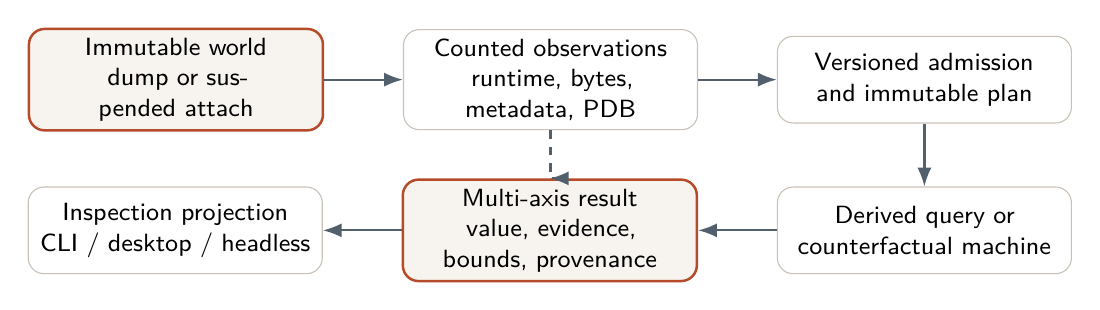
\begin{tikzpicture}[
  node distance=8mm and 10mm,
  box/.style={draw=PhoenixRule,rounded corners=2mm,fill=white,minimum height=11mm,text width=35mm,align=center,font=\small\sffamily},
  strong/.style={box,draw=PhoenixOrange,line width=0.9pt,fill=PhoenixPaper},
  arrow/.style={-{Latex[length=2.4mm]},line width=0.8pt,draw=PhoenixMuted}
]
  \node[strong] (world) {Immutable world\\dump or suspended attach};
  \node[box,right=of world] (obs) {Counted observations\\runtime, bytes, metadata, PDB};
  \node[box,right=of obs] (plan) {Versioned admission\\and immutable plan};
  \node[box,below=of plan] (eval) {Derived query or\\counterfactual machine};
  \node[strong,left=of eval] (result) {Multi-axis result\\value, evidence, bounds, provenance};
  \node[box,left=of result] (host) {Inspection projection\\CLI / desktop / headless};
  \draw[arrow] (world) -- (obs);
  \draw[arrow] (obs) -- (plan);
  \draw[arrow] (plan) -- (eval);
  \draw[arrow] (eval) -- (result);
  \draw[arrow] (result) -- (host);
  \draw[arrow,dashed] (obs.south) |- (result.north);
\end{tikzpicture}
\caption{The repository's recurring control-flow shape. Evidence is acquired before it is composed; the final result retains both the composition and its physical inputs.}
\label{fig:core-shape}
\end{figure}

\section{Milestone names embedded in the code}

Many comments and diagnostic codes use W1--W8 labels. They are historical vertical slices rather than namespaces of a clean-sheet architecture:

\begin{longtable}{L{17mm}L{39mm}L{89mm}}
\toprule
\textbf{Slice} & \textbf{Center of gravity} & \textbf{Lasting architectural contribution} \\
\midrule
\endfirsthead
\toprule
\textbf{Slice} & \textbf{Center of gravity} & \textbf{Lasting architectural contribution} \\
\midrule
\endhead
W1 & Method-body evidence & Content identities, typed metadata/body acquisition, evidence comparison. \\
W2 & Rooted field query & Parse once, select once, immutable object-specific plan, derived-query result. \\
W3 & Concrete IL execution & Domain-parametric machine, persistent memory, structural handles. \\
W4 & Counterfactual method evaluation & Whole-call-graph preparation, private plan issuance, provenance-bearing execution result. \\
W5 & Expression routing & One product entry path that preserves distinct W2 and W4 contracts. \\
W6 & Member chains & Versioned project-owned chain admission and hop-by-hop evidence composition. \\
W7 & Static-field expressions & Metadata authority, runtime declaration mapping, frame/PDB context, storage observations. \\
W8 & Static-field V2 authority work & Source-anchored metadata catalogs, complete-table discipline, broader binding and conformance machinery. \\
\bottomrule
\end{longtable}

Later work, notably the E1--E7 Edit-and-Continue plan, builds on those surfaces. A class retaining a W4 or W7 name should therefore be read as an intentionally frozen contract boundary, not as evidence that the overall product stopped at that milestone.

\begin{sourcebox}
Start with \repoPath{README.md}, \repoPath{docs/proposals/architecture/architecture-overview-proposal.md}, and then the public contracts in \repoPath{src/PhoenixInspect.Core.Abstractions}. The README explains the user-visible surface; the architecture proposal explains the truth model; the contracts show which parts are enforced by code.
\end{sourcebox}


\chapter{Repository map, build system, and dependency direction}
\label{ch:repo-map}

\section{Top-level geography}

The repository is arranged around executable evidence rather than around a single application:

\begin{description}[style=nextline]
  \item[\repoPath{src/}] Thirteen production projects: core contracts and execution, concrete validation domain, metadata contracts and SRM backend, host contracts and ClrMD adapter, product query/debugging facades, a shared inspection/presentation layer, a headless reference consumer, and CLI/desktop hosts.
  \item[\repoPath{tests/}] Unit tests, integration tests, dump-generating fixture targets, optimized-build targets, W7/W8 shape fixtures, and the Edit-and-Continue target. Fixtures are part of the evidence apparatus, not incidental sample code.
  \item[\repoPath{samples/}] The deterministic \repoPath{Contoso.OrderService} preview scenario used to produce a narrated, reproducible incident dump.
  \item[\repoPath{docs/}] Product guides, architecture proposals, milestone history, evidence dispositions, and future-work plans. Some status prose is historical and can lag the exact implementation during an active research sequence; commit-pinned code and the active plan take precedence.
  \item[\repoPath{eng/}] Headless wrappers, preview-demo automation, documentation checks, and repository governance scripts.
  \item[Root build files] \repoPath{PhoenixInspect.sln}, \repoPath{global.json}, \repoPath{Directory.Build.props}, \repoPath{Directory.Packages.props}, lock files, and the CI workflow.
\end{description}

\section{The production project graph}

The dependency direction is one of the clearest explanations of the design. Figure~\ref{fig:project-deps} emphasizes the layering; Appendix~\ref{app:projects} records exact direct references. Lower layers know nothing about dumps or user interfaces. The presentation projects know about immutable display projections, not analysis internals. The product facades sit between physical adapters and hosts.

\begin{figure}[htbp]
\centering
\begin{tikzpicture}[
  band/.style={draw=PhoenixRule,rounded corners=1.7mm,fill=white,text width=139mm,minimum height=11mm,align=center,font=\small\sffamily,inner xsep=3mm,inner ysep=2mm},
  edge/.style={-{Latex[length=2mm]},draw=PhoenixMuted,line width=0.7pt}
]
\node[band,fill=orange!3,draw=PhoenixGold] (hosts) {
  \textbf{Hosts and public consumers}\\[-0.3mm]
  \repoPath{PhoenixInspect.Cli}\quad
  \repoPath{PhoenixInspect.Desktop}\quad
  \repoPath{Headless.ReferenceConsumer}
};
\node[band,below=5mm of hosts,fill=orange!2,draw=PhoenixGold] (inspection) {
  \textbf{Host-neutral presentation and session ownership}\\[-0.3mm]
  \repoPath{PhoenixInspect.Inspection}
};
\node[band,below=5mm of inspection,fill=green!3,draw=PhoenixGreen] (products) {
  \textbf{Product semantics and admission}\\[-0.3mm]
  \repoPath{Product.DumpDebugging}\quad
  \repoPath{Product.DumpQuery}
};
\node[band,below=5mm of products,fill=blue!3,draw=PhoenixBlue] (adapters) {
  \textbf{Physical and artifact authority}\\[-0.3mm]
  \repoPath{Host.Dump.ClrMD}\quad
  \repoPath{Metadata.SRM}
};
\node[band,below=5mm of adapters,fill=PhoenixPaper,draw=PhoenixOrange] (foundation) {
  \textbf{Foundational contracts, execution, and concrete semantics}\\[-0.3mm]
  \repoPath{Core.Abstractions}\quad
  \repoPath{Core.Execution}\quad
  \repoPath{Domain.Concrete}\\[-0.3mm]
  \repoPath{Host.Abstractions}\quad
  \repoPath{Metadata.Abstractions}
};
\draw[edge] (hosts) -- (inspection);
\draw[edge] (inspection) -- (products);
\draw[edge] (products) -- (adapters);
\draw[edge] (adapters) -- (foundation);
\draw[edge,dashed] ([xshift=48mm]hosts.south) to[out=-25,in=25] ([xshift=48mm]products.north);
\end{tikzpicture}
\caption{Layered production dependency direction. The dashed shortcut represents the headless consumer's direct use of product APIs; Appendix~\ref{app:projects} lists every exact project reference.}
\label{fig:project-deps}
\end{figure}

\subsection{Project responsibilities}

\begin{longtable}{L{48mm}L{101mm}}
\toprule
\textbf{Project} & \textbf{Responsibility} \\
\midrule
\endfirsthead
\toprule
\textbf{Project} & \textbf{Responsibility} \\
\midrule
\endhead
\repoPath{PhoenixInspect.Core.Abstractions} & Immutable identities, structural type/signature vocabulary, result axes, canonical replay encoding, value-domain and memory-model interfaces, resolution and provenance contracts. \\
\repoPath{PhoenixInspect.Core.Execution} & Whole-method-graph preparation and the deterministic, domain-parametric IL machine. \\
\repoPath{PhoenixInspect.Domain.Concrete} & Lifted-flat concrete values, persistent concrete memory, and provenance-enriched concrete semantics used to validate and productize the execution core. \\
\repoPath{PhoenixInspect.Host.Abstractions} & Snapshot byte-reading contracts that distinguish exact, short, and unavailable reads. \\
\repoPath{PhoenixInspect.Metadata.Abstractions} & Bounded metadata-module capabilities and path-independent module descriptions. \\
\repoPath{PhoenixInspect.Metadata.SRM} & The \typeName{System.Reflection.Metadata}/PE implementation of those metadata contracts, separated into acquisition and projection. \\
\repoPath{PhoenixInspect.Host.Dump.ClrMD} & ClrMD lifetime, module/runtime catalogs, raw memory, heap and field observations, frame/PDB evidence, method-body acquisition, static storage, live attach, and typed adapter outcomes. \\
\repoPath{PhoenixInspect.Product.DumpQuery} & Roslyn parsing and project-owned admission, rooted queries, member chains, static-field binding/evaluation, the deterministic expression evaluator, metadata-authority catalogs, and edit-generation contracts. \\
\repoPath{PhoenixInspect.Product.DumpDebugging} & Unified expression routing for method paths, dump-method acquisition, counterfactual memory/import, preparation, execution, and canonical result projection. \\
\repoPath{PhoenixInspect.Headless.ReferenceConsumer} & Executable public-contract witness, usefulness portfolios, corpus replay, and golden/conformance output independent of a UI. \\
\repoPath{PhoenixInspect.Inspection} & Host-neutral session ownership, immutable display models, evaluation reporting, completion, process discovery, and source navigation. It adds presentation policy, not analysis semantics. \\
\repoPath{PhoenixInspect.Cli} & Scriptable and interactive console host, dump capture command, transcript renderer, command/session state. \\
\repoPath{PhoenixInspect.Desktop} & Avalonia docked debugger-style shell, MVVM state, Watch/Immediate/source panes, and visual interaction. \\
\bottomrule
\end{longtable}

\begin{takeaway}
The apparently odd split between \repoPath{Product.DumpQuery} and \repoPath{Product.DumpDebugging} is intentional. The former owns read-only binding and derived-query semantics; the latter imports those facts into the IL interpreter and preserves counterfactual semantics. Merging them would make it easier to accidentally present interpreted behavior as observed state.
\end{takeaway}

\section{Build configuration}

The repository pins the .NET SDK to 10.0.201 with latest-patch roll-forward and disallows prerelease SDK selection. Shared build properties establish:

\begin{itemize}
  \item target framework \codeinline{net10.0};
  \item C\# 14;
  \item nullable reference types and implicit global usings;
  \item deterministic builds and XML documentation;
  \item package lock files everywhere and locked restore in CI;
  \item warnings as errors in CI rather than necessarily during every local exploratory build.
\end{itemize}

A second \repoPath{src/Directory.Build.props} scopes product versioning (\codeinline{0.1.0-preview.1}) to shipping projects. Keeping fixture assemblies outside that version injection is significant: fixture identity is evidence, so incidental product-version changes must not silently perturb the binaries and dumps used as controls.

Central package management fixes the major moving parts: ClrMD 4.0, the diagnostics client, Roslyn 5.3.0, Avalonia 12.1, Dock, AvaloniaEdit, ProDataGrid, ILSpy/decompiler 9.1, and the xUnit/test infrastructure. The parser also records the Roslyn package version in its own profile identity; the dependency version is therefore part of semantics, not merely a build detail.

\section{CI as an evidence matrix}

The workflow is split by what each lane proves:

\begin{description}[style=nextline]
  \item[Documentation lane] Runs link validation and a guard that checks the documented headless workflow. This prevents the architectural narrative from becoming completely detached from executable entry points.
  \item[Fast Windows lane] Locked restore, Release build, unit tests, and the fast integration category.
  \item[Real dump evidence lane] Generates/opens ordinary fixture dumps and exercises adapter/product paths against actual captured state.
  \item[Preview demo lane] Executes the end-to-end sample workflow and publishes the narrated transcript as an artifact.
  \item[Optimized-context lane] Uses a Release/optimized target to prove behavior where debugger context is incomplete or transformed by optimization.
\end{description}

The latest commit record for \shortcommit reports 1,327 unit tests, 629 fast integration tests, 12 Edit-and-Continue fixture tests, four focused delta-acquisition tests, and zero skips for the cited closure runs. Those are commit-recorded verification facts, not independent measurements made while producing this document.

\section{Running the code}

The shortest user-facing path is the preview script:

\begin{lstlisting}[language={},numbers=none]
./eng/Invoke-PreviewDemo.ps1
\end{lstlisting}

To inspect an existing dump through the CLI:

\begin{lstlisting}[language={},numbers=none]
dotnet run --project src/PhoenixInspect.Cli -- <path-to-your.dmp>
\end{lstlisting}

The CLI also accepts a suspended live attach, repeated \codeinline{--eval} or \codeinline{--command} arguments, a script file, verbose evidence, and color suppression. The desktop project uses the same \repoPath{PhoenixInspect.Inspection} services, so the choice of host does not select a different evaluator.

\section{Status documents versus exact code}

A research repository can legitimately contain several time scales. At this baseline, portions of the top-level README still describe W8.2 as active, while the exact tree and recent plan history already contain completed E1--E3 Edit-and-Continue work and name E4 as the next stride. The correct reading order for a current-state question is:

\begin{enumerate}
  \item exact commit-pinned code and tests;
  \item the active plan's status paragraphs and closure commit;
  \item milestone history/evidence dispositions;
  \item general README status prose.
\end{enumerate}

The older text remains useful as architectural history. It should not be silently ``corrected'' when documenting a past milestone, but a current walkthrough must call out the skew.

\begin{sourcebox}
Build and dependency landmarks: \repoPath{global.json}, \repoPath{Directory.Build.props}, \repoPath{src/Directory.Build.props}, \repoPath{Directory.Packages.props}, \repoPath{PhoenixInspect.sln}, and \repoPath{.github/workflows/ci.yml}.
\end{sourcebox}

\chapter{The core contract language}
\label{ch:contracts}

\section{Why the abstractions project is the center of gravity}

\repoPath{PhoenixInspect.Core.Abstractions} contains no dump reader and no execution loop, yet it is the most important project for understanding repository-wide behavior. It defines what can be claimed. The rest of the system either produces these claims, transforms them, or displays them.

Its contents fall into five families:

\begin{enumerate}
  \item structural identities and handles for artifacts, modules, methods, fields, objects, and source worlds;
  \item a bounded ECMA-335 type/signature vocabulary;
  \item multi-axis evaluation results, diagnostics, provenance, evidence context, and deterministic bounds;
  \item replay/canonical-encoding primitives;
  \item capability interfaces for value domains, memory, budgets, metadata resolution, and pure-call models.
\end{enumerate}

This arrangement prevents lower-level mechanics from inventing ad hoc meanings. A short memory read, ambiguous metadata match, unsupported signature, budget stop, and invalid program are different facts before any host sees them.

\section{Result axes: no single status can tell the truth}

The generic \typeName{EvaluationResult<T>} is best understood as a product type rather than a success/failure union. Its principal axes are independent, subject to coherence constraints.

\begin{longtable}{L{33mm}L{42mm}L{70mm}}
\toprule
\textbf{Axis} & \textbf{Representative values} & \textbf{Question answered} \\
\midrule
\endfirsthead
\toprule
\textbf{Axis} & \textbf{Representative values} & \textbf{Question answered} \\
\midrule
\endhead
Semantic mode & Observation; DerivedQuery; CounterfactualExecution; AbstractAnalysis & What kind of truth is being claimed? \\
Completion & Completed; Blocked; BudgetExhausted; Cancelled; Invalid & Why did the operation stop? \\
Completeness & Complete; Partial; None & How much semantic answer exists? \\
Evidence & Exact; Partial; Unavailable; Conflict; Invalid & How strong and coherent were the physical inputs? \\
Effects & None; VirtualOnly; Modeled; Unsupported & What effect semantics were admitted? \\
Value & Optional typed value & Is there a semantic value, prefix, or witness to carry? \\
Provenance & DumpMemory; RuntimeStructure; Artifact; Policy; Transformation & Which sources and transformations support the answer? \\
Diagnostics & Stable code plus artifact-independent message & What named disposition explains a non-ideal outcome? \\
Reached bounds & Named deterministic limits actually encountered & Which finite policy gates materially constrained the operation? \\
\bottomrule
\end{longtable}

Consider three superficially similar ``no ordinary value'' outcomes:

\begin{itemize}
  \item a syntactically valid but unsupported expression: completion may be \status{Blocked}, completeness \status{None}, evidence \status{Exact}; the parser knows exactly that the admitted profile excludes it;
  \item a field read whose dump bytes are truncated: completion \status{Blocked}, completeness \status{None} or \status{Partial}, evidence \status{Partial};
  \item a cancelled method interpretation after several transfers: completion \status{Cancelled}, completeness \status{Partial}, value an execution-prefix witness, and exact/partial evidence aggregated from the observations already consumed.
\end{itemize}

Flattening all three to ``error'' would lose the information PhoenixInspect exists to preserve.

\subsection{Constructor-enforced coherence}

The result constructor validates cross-axis invariants. In schematic form:

\begin{lstlisting}[caption={Representative coherence rules enforced by the result contract. This is schematic rather than a verbatim source extract.}]
if (mode is Observation or DerivedQuery)
    require effects == None;

if (completeness is Complete or Partial)
    require value is present;

if (completeness == None)
    require value is absent;

if (completion != Completed)
    forbid completeness == Complete;
\end{lstlisting}

The important architectural consequence is that a malformed result cannot travel far. A product facade cannot claim a complete value after cancellation, and a derived query cannot accidentally announce virtual side effects, without failing at construction.

\section{Evidence context}

\typeName{EvaluationEvidenceContext} records the identity and finite policy envelope surrounding a result. Its source kind distinguishes no external source, a dump snapshot, an artifact, or synthetic evidence. Identity availability is itself explicit: \status{Available}, \status{Unavailable}, or \status{NotApplicable}. This avoids the common ambiguity where a null digest could mean either ``not needed'' or ``needed but missing.''

Fallback is similarly explicit. The context says either that no fallback occurred or names the fallback that did. If a disk assembly was used only after its content identity matched the dump module, that transformation belongs in provenance; it is not an invisible implementation convenience.

Only bounds actually reached are retained. A configured maximum that played no role in an operation is not evidence about the outcome. This keeps replay identity stable and reports readable while still making cap-induced incompleteness auditable.

\begin{invariantbox}
A result over a dump snapshot must name the snapshot identity. Where module identity is relevant, the context must state either the exact module identity or an explicit unavailable outcome. ``We happened not to populate the field'' is not an admissible third state.
\end{invariantbox}

\section{Stable diagnostics}

Diagnostics consist of a stable code and an artifact-independent explanation. Paths, exception payloads, arbitrary parser text, and target-specific display strings are excluded from canonical identity. Hosts may add contextual presentation around the diagnostic, but the product code remains suitable for replay and golden comparison.

The code families also reveal pipeline ownership: \codeinline{META_*} for metadata admission, \codeinline{DUMP_*} for host evidence, \codeinline{QUERY_*} for rooted query syntax/evaluation, \codeinline{W4.*} for counterfactual preparation/execution, and newer W7/W8 or Edit-and-Continue dispositions for those staged contracts. The names are intentionally more precise than an exception type.

\section{Identity is content first, location second}

Several identity types coexist because they answer different questions:

\begin{description}[style=nextline]
  \item[\typeName{ArtifactContentIdentity}] Is this complete external file byte-for-byte the same artifact?
  \item[\typeName{ModuleContentIdentity}] Does this metadata content, anchored by MVID and metadata bytes, identify the same logical module content?
  \item[\typeName{ModuleId}] What module identity results from content identity, PE stamp, and artifact identity?
  \item[\typeName{ModuleHandle}] What compact structural identity should the execution core use without knowing paths or SRM objects?
  \item[\typeName{MethodHandle}/\typeName{FieldHandle}] Which metadata definition in which structural module is referenced?
  \item[Snapshot identity] Which captured world supplied this address, runtime object, or frame?
\end{description}

Paths remain in descriptors and display provenance. They can help locate a candidate artifact but never prove that candidate. This is why copying an assembly or dump does not change its stable identity, while replacing a file at the same path does.

\subsection{Atomic observations prevent time-slice mixtures}

\typeName{IMetadataModule.GetMethodDefinition} returns body and activation shape as one immutable observation. The alternative---fetching a body, then separately fetching signature and locals---would permit callers to combine facts acquired from different effective generations or sources. The interface still exposes a body-only compatibility operation for W1 evidence comparison, but interpreter activation is required to use the atomic definition.

This distinction becomes especially important in the Edit-and-Continue work, where a base-image body and a generation-aware signature would be individually plausible yet jointly false.

\section{Canonical replay encoding}

\typeName{CanonicalReplayEncoding} is a small serialization protocol whose job is not interchange convenience but deterministic identity. A writer begins with a domain string and positive schema version, then emits:

\begin{itemize}
  \item integers in an explicitly chosen big-endian representation;
  \item length-prefixed byte sequences;
  \item strings as counted UTF-16 code units rather than environment-dependent text encodings;
  \item normalized digest text and bounded vectors in deterministic order.
\end{itemize}

The resulting bytes are hashed with SHA-256. Equality for many immutable contracts compares canonical bytes, and deterministic hash codes derive from the digest rather than object identity.

\begin{figure}[htbp]
\centering
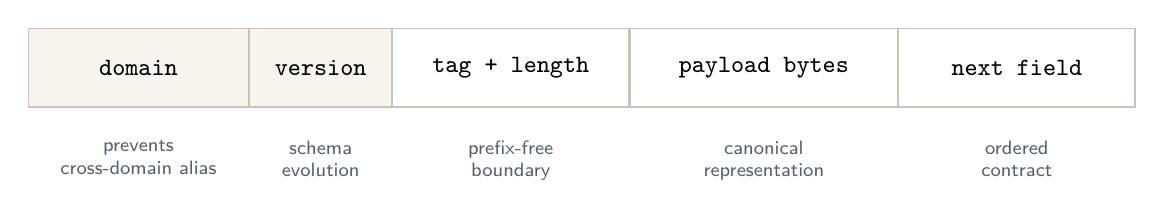
\begin{tikzpicture}[
  seg/.style={draw=PhoenixRule,minimum height=10mm,align=center,font=\small\ttfamily},
  note/.style={font=\scriptsize\sffamily,align=center,text=PhoenixMuted}
]
\node[seg,fill=PhoenixPaper,minimum width=28mm] (domain) {domain};
\node[seg,fill=PhoenixPaper,minimum width=18mm,right=0pt of domain] (ver) {version};
\node[seg,minimum width=30mm,right=0pt of ver] (field1) {tag + length};
\node[seg,minimum width=34mm,right=0pt of field1] (payload1) {payload bytes};
\node[seg,minimum width=30mm,right=0pt of payload1] (field2) {next field};
\node[note,below=3mm of domain] {prevents\\cross-domain alias};
\node[note,below=3mm of ver] {schema\\evolution};
\node[note,below=3mm of field1] {prefix-free\\boundary};
\node[note,below=3mm of payload1] {canonical\\representation};
\node[note,below=3mm of field2] {ordered\\contract};
\end{tikzpicture}
\caption{Conceptual shape of canonical contract encoding. The exact writer API is typed, but every sequence is domain-separated, versioned, and prefix-free.}
\end{figure}

\subsection{Compatibility discipline}

Canonical encodings are treated as compatibility surfaces. Additive fields are normally appended behind a distinct tag or absence-preserving representation so an old zero-feature case remains byte-identical. The Edit-and-Continue work repeatedly tests this requirement: a zero-generation module must keep existing W1--W8 digests unchanged.

A change that merely preserves object equality but changes canonical bytes is therefore not harmless. It can invalidate replay identity, goldens, corpus reports, and cross-run comparison.

\section{The ECMA-335 type and signature vocabulary}

The core contracts include a bounded structural grammar for CLI types and signatures rather than leaking \typeName{System.Type}, SRM handles, or reflection objects into execution. Representative shapes include primitive stack kinds, named value/reference types, arrays, pointers/byrefs where admitted, generic parameters and instantiations, and method/local/field signatures.

The large \repoPath{BoundedEcmaSignatureProjection.cs} implementation performs counted, closed-profile decoding. It is intentionally not a permissive ECMA metadata parser. Unsupported constructs remain typed unsupported results; malformed encodings remain invalid; recursion, node count, and token resolution are bounded.

This has three benefits:

\begin{enumerate}
  \item metadata backends can change while execution identities stay structural;
  \item tests can generate and compare signatures without loading assemblies;
  \item the machine can validate stack and argument shapes without depending on reflection or the host runtime.
\end{enumerate}

\section{Capability interfaces}

\subsection{\typeName{IValueDomain<TValue>}}

The value domain supplies lattice and execution semantics: bottom/top, constants, join/meet/widen, partial order, static type and stack kind, exact-value extraction, and the admitted arithmetic operations. The machine does not know whether a value is concrete, abstract, provenance-wrapped, or symbolic.

This is more than generic-programming elegance. It separates the IL transfer relation from the precision policy. The same instruction can produce an exact integer in the concrete domain or an explained unknown in another domain without changing the machine's control-flow code.

\subsection{\typeName{IMemoryModel<TValue,TMemory>}}

Memory is persistent: reads return a typed \typeName{MemoryLoadResult}; writes return descendant snapshots. The contract explicitly forbids turning missing dump evidence into default field values. A zero-initialized virtual allocation and an unavailable captured field are semantically different and must remain distinguishable.

\subsection{Resolution and models}

Resolution services translate structural handles and tokens into admitted method/field definitions. Pure-call model registries provide explicit, versioned replacements for selected helpers. Model selection occurs during graph preparation, before execution and, where required, before acquiring a target body. That order ensures the frozen graph says exactly which capability will answer each call site.

\section{A practical rule for reading contracts}

When a class seems to carry ``too many'' fields, classify them into four groups:

\begin{enumerate}
  \item semantic payload;
  \item identity/replay payload;
  \item physical evidence and provenance;
  \item finite-policy accounting.
\end{enumerate}

Most apparent redundancy disappears. For example, a result may retain both a selected field descriptor and raw read evidence because the former says \emph{what was selected} while the latter says \emph{what bytes made the value available}.

\begin{sourcebox}
Read these files together: \repoPath{EvaluationResult.cs}, \repoPath{EvaluationEvidenceContext.cs}, \repoPath{CanonicalReplayEncoding.cs}, \repoPath{IValueDomain.cs}, \repoPath{IMemoryModel.cs}, and \repoPath{BoundedEcmaSignatureProjection.cs}. The unit suites \repoPath{EvaluationResultTests.cs}, \repoPath{CanonicalReplayEncodingTests.cs}, and \repoPath{BoundedEcmaSignatureProjectionTests.cs} are the quickest executable specification of edge cases.
\end{sourcebox}


\chapter{Whole-graph planning and the deterministic IL machine}
\label{ch:execution}

\section{Preparation and execution are separate protocols}

The execution core does not accept an arbitrary method handle and resolve as it goes. \typeName{MethodGraphPlanner} first discovers, validates, and freezes the complete admitted direct-call closure. \typeName{IlMachine<TValue,TMemory>} then executes only that frozen graph. This separation is the execution analogue of parse-once/select-once query planning.

\begin{figure}[htbp]
\centering
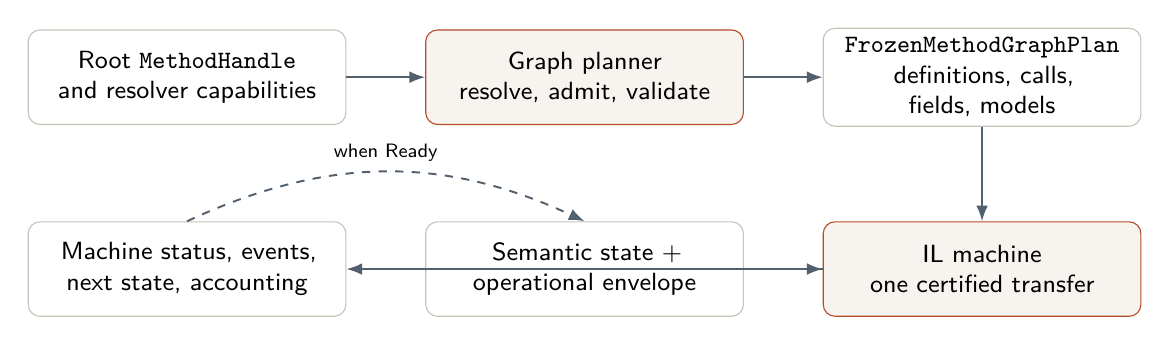
\begin{tikzpicture}[
  box/.style={draw=PhoenixRule,rounded corners=1.5mm,fill=white,text width=38mm,minimum height=12mm,align=center,font=\small\sffamily},
  gate/.style={box,fill=PhoenixPaper,draw=PhoenixOrange},
  edge/.style={-{Latex[length=2mm]},draw=PhoenixMuted,line width=0.7pt}
]
\node[box] (root) {Root \typeName{MethodHandle}\\and resolver capabilities};
\node[gate,right=10mm of root] (planner) {Graph planner\\resolve, admit, validate};
\node[box,right=10mm of planner] (graph) {\typeName{FrozenMethodGraphPlan}\\definitions, calls, fields, models};
\node[gate,below=12mm of graph] (machine) {IL machine\\one certified transfer};
\node[box,left=10mm of machine] (state) {Semantic state +\\operational envelope};
\node[box,left=10mm of state] (outcome) {Machine status, events,\\next state, accounting};
\draw[edge] (root) -- (planner);
\draw[edge] (planner) -- (graph);
\draw[edge] (graph) -- (machine);
\draw[edge] (state) -- (machine);
\draw[edge] (machine) -- (outcome);
\draw[edge,bend left=25,dashed] (outcome.north) to node[above,font=\scriptsize\sffamily]{when Ready} (state.north);
\end{tikzpicture}
\caption{The plan/execute split. No metadata or call-target resolution is permitted in the execution loop.}
\label{fig:plan-execute}
\end{figure}

The planner's output is not simply a cache. It is an admission certificate: every reachable body, signature, local, field operand, call target, model selection, and required logical depth has already passed a closed set of checks.

\section{Graph traversal and accounting}

Planning performs root-first depth-first traversal, visiting call sites in increasing IL offset. Public vectors are later canonicalized by structural identity so replay does not depend on incidental dictionary order. A fresh first-result cache is scoped to one preparation attempt, which prevents a previous request's failure or capability observation from contaminating another request.

The traversal has explicit limits, including a product-level traversal-unit budget and an internal method-count cap. Importantly, a zero traversal limit stops before invoking resolver or model-registry capabilities. Tests verify not only the final disposition but which capability calls were avoided.

Each potential operation is charged according to a frozen accounting rule. When a bound is crossed, the failure retains the first rejected charge and the traversal prefix rather than pretending no work occurred.

\subsection{Model selection before body acquisition}

For an optional required pure model, the planner identifies the exact target and selects the model before asking for that callee's body. This ordering serves two purposes:

\begin{itemize}
  \item the model is a declared semantic replacement, not a fallback after body acquisition happened to fail;
  \item a modeled external/helper call can be admitted without granting unnecessary body-reading authority.
\end{itemize}

An interpreted-only request never queries the optional model registry. Capability non-use is part of the contract and is tested.

\section{Machine state versus operational state}

The machine maintains two parallel envelopes:

\begin{description}[style=nextline]
  \item[Semantic state] Call stack, frame arguments/locals/evaluation stack, persistent memory, root return value, and terminal target-exception state.
  \item[Operational state] Remaining instruction budget, configured and observed logical depth, active-frame high-water marks, pure-model attempts, invocation counts, and completed modeled-call counts.
\end{description}

Separating them prevents budget instrumentation from changing semantic equality and makes ``no instruction executed'' assertions precise. A budget-exhausted transfer returns the exact same semantic state and operational object when the pre-instruction budget is zero.

\section{The admitted IL profile}

The current machine is intentionally a closed, scenario-derived subset rather than a partial implementation that silently mishandles the rest of ECMA-335. Its concrete path includes the operations needed by the proven fixture corpus: integer constants and arguments, initialized locals, selected arithmetic, ordinary instance field loads, control-neutral \codeinline{nop}, return, direct admitted calls, and pure modeled calls. Additional functionality is split between transfer files and the prepared-graph implementation, but every opcode must have explicit validation, stack behavior, event behavior, accounting, and tests.

Unsupported opcode or signature shapes fail during planning where possible. Invalid stack behavior and malformed bodies remain invalid-program outcomes. Unknown continuation is admitted only under an explicit \typeName{UnknownExecutionPolicy} and only when the value domain exposes the needed capability.

\begin{warningbox}
Do not infer full CLR semantics from the generic class name \typeName{IlMachine}. It is a deterministic machine for a closed profile. The design makes extending that profile disciplined; it does not claim that an unimplemented opcode can be approximated safely.
\end{warningbox}

\section{Activation}

Prepared activation verifies the root method, required logical depth, receiver/argument vector, static types, locals, and initial memory identity. It creates one root frame at IL offset zero with an empty evaluation stack and default-initialized locals according to the admitted semantics. Activation consumes no instruction budget.

The counterfactual runner later revalidates this state: exactly one root frame, no return value, no terminal exception, same persistent memory identity, matching root method, and exact reference retention for the materialized argument vector.

\section{One instruction is one certified transition}

\typeName{StepOne} returns a \typeName{StepOutcome} stamped by the machine for the exact prior semantic and operational envelopes. The product runner verifies that stamp before trusting any result. Successful ordinary transfers:

\begin{itemize}
  \item consume exactly one instruction unit;
  \item produce an \typeName{InstructionExecuted} event, optionally followed by one frame or precision event;
  \item preserve persistent memory identity for the current read-only rooted product path;
  \item change call-stack depth only as announced by a frame event;
  \item preserve or extend model-attempt accounting by at most one coherent entry.
\end{itemize}

Blocked and invalid transfers change neither semantic state nor budget and emit no ordinary events. Target exceptions have their own terminal union and event shape. The runner treats a violation of these internal contracts as a replay-invalid result rather than accepting a plausible next state.

\section{Terminal idempotence}

After a completed root return, the runner calls \typeName{StepOne} once more and requires an idempotent terminal transition. It also checks that no field load, provenance node, budget, event, or model counter changed. This is a compact but powerful replay guarantee: terminal state is not merely recognized by one control branch; it is stable under the machine's public stepping protocol.

\section{Budgets and finite execution}

The machine's instruction budget is caller-configured within product limits. The runner also calculates a graph-derived finite dynamic instruction bound for the acyclic prepared graph and caps the number of step requests at the lesser of that cost and the instruction budget, plus the mandatory terminal check. Exceeding that bound is treated as internal invalidity: the frozen graph and transfer accounting promised finiteness.

Logical call depth is separate from active frame depth. A pure model may enter logical depth without creating an interpreted frame, so both high-water marks are retained. Preparation rejects a configured logical-depth limit smaller than the graph's required depth before any instruction executes.

Cancellation is observed only at ready machine boundaries. A terminal transfer and its required idempotence check take precedence over cancellation arriving after completion. A cancelled run with no executed instruction carries no semantic value; a cancelled run after progress can carry an execution-prefix value and partial completeness.

\section{Events and provenance}

Debug events are not a UI log pasted onto execution. They are part of the transition contract and canonical result. Representative events describe instructions, frame pushes/pops, value precision loss, and target exceptions. Field-load evidence and provenance lineage connect values back to captured observations and transformations.

Exact primitive values can bypass expensive lineage structures where no explanation is needed. Explained unknowns require provenance capability so the product can report why precision was lost instead of returning an opaque top value.

\section{Failure taxonomy}

A useful debugging distinction is where a failure occurred:

\begin{description}[style=nextline]
  \item[Resolution/admission failure] The graph could not be completely frozen. No partial executable plan escapes.
  \item[Request/binding failure] Receiver, arguments, evidence, policy, or memory/domain capabilities are mutually incompatible.
  \item[Activation failure] A supposedly valid plan could not produce the exact initial machine state.
  \item[Blocked transfer] A required admitted runtime capability was unavailable at one instruction boundary.
  \item[Invalid program/transition] IL or a capability result contradicted the closed machine contract.
  \item[Budget/cancellation] Finite host policy ended an otherwise coherent run.
  \item[Target exception] The modeled target semantics produced an exception; the current non-null rooted facade has deliberately narrow handling for this case.
\end{description}

Because each stage has typed output, a test can assert that a malformed call signature never reaches activation, or that zero traversal never touches a resolver, rather than merely observing a final error code.

\begin{sourcebox}
Core execution landmarks: \repoPath{MethodGraphPlanner.cs}, \repoPath{MethodPlanBuilder.cs}, \repoPath{FrozenMethodGraphPlan.cs}, \repoPath{IlMachine.cs}, \repoPath{IlMachine.PreparedGraph.cs}, and \repoPath{IlMachine.Transfers.cs}. The deepest behavioral specifications are \repoPath{MethodGraphPlannerTests.cs}, \repoPath{MethodGraphPlannerTraversalAccountingTests.cs}, \repoPath{IlMachineTests.cs}, \repoPath{PreparedGraphExecutionTests.cs}, and \repoPath{PreparedGraphModelExecutionTests.cs}.
\end{sourcebox}


\chapter{Concrete values, persistent memory, and provenance}
\label{ch:domain}

\section{The concrete domain is a lifted-flat validation domain}

\repoPath{PhoenixInspect.Domain.Concrete} supplies the domain used by current counterfactual product paths. Its lattice is intentionally simple and mechanically testable. For a fixed static type, the ordering is essentially

\[
  \bot \;\sqsubseteq\; c \;\sqsubseteq\; \top,
\]

where each exact constant \(c\) is incomparable with a distinct exact constant. Consequently:

\begin{itemize}
  \item joining an exact value with itself preserves it;
  \item joining distinct exact values yields unknown/top;
  \item meeting distinct exact values yields bottom;
  \item bottom joins to the other operand and top meets to the other operand;
  \item widening is predictable because the domain has no ascending numeric intervals.
\end{itemize}

This is not intended to be the final abstract-analysis domain. It is the smallest domain that can validate transfer semantics, preserve exact fixture values, and represent explained loss of precision.

\section{Value shapes}

\typeName{ConcreteValue} represents exact primitive values and deterministic structural references admitted by the machine. Integer operations use the intended unchecked Int32/Int64 semantics where the opcode profile calls for them. Object and array references are identities in virtual/captured memory, not analysis-process object references.

Static type and CLI stack kind are kept explicit. A value that is structurally Int32 cannot be substituted for a reference simply because both are stored in one C\# union type. Argument and field-load validation use those shapes before execution.

\section{Persistent memory}

\typeName{ConcreteMemory} is an immutable snapshot. \typeName{ConcreteMemoryModel} reads and returns either exact values or typed non-exact loads; writes construct descendant snapshots. Persistence has several consequences:

\begin{itemize}
  \item a plan can retain its exact initial memory without worrying that another run mutates it;
  \item replay comparison can use structural memory identity;
  \item virtual effects are distinguishable from captured evidence;
  \item machine states can share unchanged memory cheaply;
  \item a failed transfer can prove it preserved the exact prior memory object.
\end{itemize}

The dump product currently emphasizes read-only rooted evaluation. The persistent interface nevertheless keeps future virtual mutation and stepping semantics honest: a store never writes into the dump, and descendants are explicit.

\section{Field loads are evidence-bearing operations}

A field load is not simply \typeName{TValue?}. It can be exact, absent under a proved condition, unavailable, partial, conflicting, or invalid, with evidence and diagnostics. The memory model must not use CLI default initialization to fill a hole in captured memory. Default initialization is valid for a newly allocated virtual object whose construction semantics are known; it is not valid for a dump page that was omitted.

The counterfactual product wraps the memory model in \typeName{CounterfactualRecordingMemoryModel}. This adapter records which predeclared field observations were actually reached and in what ordinal order. Final evidence is aggregated from reached observations, not from every field the graph could theoretically access.

\section{Provenance-enriched concrete values}

\typeName{ProvenanceConcreteValue} pairs concrete precision with a lineage graph. Nodes can represent dump memory, field transfers, calls, model transformations, and precision loss. The graph is interned to keep repeated lineage structures deterministic and bounded.

The design avoids attaching a heavyweight explanation to every exact constant. Where an operation remains exact and its source is already represented by the result-level evidence, the value can remain compact. When values merge or a capability returns an explained unknown, the lineage records the cause.

\subsection{Field and call lineage}

Separate test families cover field-source lineage, field-transfer lineage, machine propagation, interpreted-call lineage, and modeled-call lineage. This granularity is useful when extending the machine: an arithmetic opcode may compute the correct number while accidentally dropping one operand's provenance. A conventional value-only test would miss that regression.

\section{Domain laws as executable architecture}

\repoPath{ConcreteDomainLawTests.cs} checks lattice identities and order relations.\par\smallskip\noindent\repoPath{ConcreteMemoryModelTests.cs} checks persistence and read/write behavior. Provenance tests check canonical lineage rather than just display strings. These suites matter because the interpreter assumes algebraic laws: if join is not idempotent or memory descendants mutate ancestors, machine-level replay guarantees collapse.

\begin{takeaway}
The concrete domain is intentionally boring mathematics. That is a virtue: it gives the product an exact baseline against which more ambitious abstract or symbolic domains can later be validated.
\end{takeaway}

\section{Where to extend the domain}

A new value category normally requires coordinated changes in four places:

\begin{enumerate}
  \item structural type/stack-kind representation in core contracts;
  \item concrete value construction, equality, and canonical representation;
  \item domain transfer semantics and exact-value extraction;
  \item memory/model and provenance tests demonstrating persistence and lineage.
\end{enumerate}

Do not add an opaque ``object'' payload holding analysis-machine instances. That would make identity, canonical replay, and target-platform semantics ambient.

\begin{sourcebox}
Read \repoPath{ConcreteValue.cs}, \repoPath{ConcreteDomain.cs}, \repoPath{ConcreteMemory.cs}, \repoPath{ConcreteMemoryModel.cs}, and the provenance wrapper/lineage files. Then read \repoPath{ConcreteDomainLawTests.cs}, \repoPath{ConcreteMemoryModelTests.cs}, and the \repoPath{Provenance*Tests.cs} families.
\end{sourcebox}

\chapter{Metadata: from PE bytes to structural authority}
\label{ch:metadata}

\section{Two projects, two responsibilities}

Metadata work is split between two projects. \repoPath{PhoenixInspect.Metadata.Abstractions} defines the bounded capability the rest of the system may rely on. \repoPath{PhoenixInspect.Metadata.SRM} implements that capability over managed PE and metadata bytes using \typeName{System.Reflection.Metadata} and \typeName{PEReader}.

The split is essential because metadata bytes can come from more than one place:

\begin{itemize}
  \item a local PE artifact opened from disk;
  \item counted metadata bytes read from dump memory;
  \item a caller-supplied Edit-and-Continue metadata delta;
  \item eventually, a generation-aware composition of base and delta tables.
\end{itemize}

Acquisition answers ``where did the bytes come from and are they complete?'' Projection answers ``what structural method, field, type, or signature do those bytes declare?'' Combining the two would force dump-backed code either to duplicate SRM semantics or to masquerade memory bytes as a file.

\section{\typeName{IMetadataModule}}

The central abstraction exposes:

\begin{itemize}
  \item a canonical path-independent \typeName{ModuleId};
  \item a non-identity \typeName{ModuleDescriptor} containing display name and artifact location evidence;
  \item a structural \typeName{ModuleHandle} for the execution core;
  \item MethodDef token validation and conversion to \typeName{MethodHandle};
  \item atomic method-definition projection, including body and activation shape;
  \item body-independent method-operand resolution;
  \item contextual same-module FieldDef resolution;
  \item a body-only compatibility read for evidence comparison.
\end{itemize}

The contract intentionally excludes name-based overload guessing, ambient assembly loading, and broad MemberRef/MethodSpec resolution from the current admitted profile. A production binder must include namespace, arity, and signature and must report conflicts rather than choose the first method with a matching simple name.

\section{Opening an SRM module}

\typeName{SrmMetadataModule} opens a managed PE through a bounded, typed path. The throwing constructor exists for named fixtures and programmer-controlled inputs. The static \typeName{Open} method maps external failures to stable resolution outcomes:

\begin{itemize}
  \item malformed or structurally invalid path --- invalid;
  \item missing/unreadable artifact --- unavailable;
  \item file larger than the deterministic external-input cap --- unsupported;
  \item malformed PE/metadata --- invalid.
\end{itemize}

It does not echo arbitrary parser or file-system exception payloads into the product result.

The module identity combines:

\begin{enumerate}
  \item complete artifact SHA-256 identity;
  \item metadata content identity derived from MVID and metadata bytes;
  \item PE timestamp and image size as a structural stamp.
\end{enumerate}

The path and filename remain in the descriptor. Byte-identical copies therefore produce the same module and execution handles.

\section{Deterministic bounds}

The backend declares hard caps, including a 512 MiB external artifact limit, 100,000 type definitions for bounded fixture lookup, 1,000,000 method definitions, bounded lookup-name length, and a 4 KiB method-body code-byte profile for the current execution slice. These limits are not hidden implementation details. Crossing one produces a named unsupported or partial disposition and, where applicable, a reached-bound record.

The simple type/method lookup helper is documented as fixture-oriented. It counts all matches and reports ambiguity. This is a recurring repository pattern: convenience APIs are explicitly scoped so they do not become accidental production binding rules.

\section{Projection versus acquisition}

\typeName{SrmMetadataProjection} contains the reusable transformation from SRM rows and signatures to PhoenixInspect structural contracts. Both disk-backed modules and dump-counted metadata can invoke the same projection logic. This is crucial for differential tests: if the dump path and disk path disagree, the discrepancy can be localized to byte acquisition or runtime mapping rather than duplicated metadata semantics.

Projection validates token kind/range, method implementation kind, signatures, local layouts, field ownership, and the closed same-module call/field profile. A successful \typeName{ResolvedMethodDefinition} is therefore an activation-ready observation, not a thin wrapper around an SRM handle.

\section{Metadata authority in the dump-query product}

Static-field binding requires more than the minimal method-oriented \typeName{IMetadataModule}. \repoPath{PhoenixInspect.Product.DumpQuery} contains a larger source-anchored authority system: complete-table catalogs, declaration identities, ownership chains, type ancestry, signatures, constraints, imports, aliases, and binding outcomes. The W8 work emphasizes complete physical tables and canonical source correlation rather than ``find a row that looks right.''

The authority pipeline generally follows this order:

\begin{enumerate}
  \item acquire complete counted metadata bytes for a runtime module instance;
  \item produce physical table catalogs retaining row order, row counts, and source identity;
  \item project definition identities and ownership/ancestry relationships;
  \item bind a parsed spelling under a closed contextual or fully qualified route;
  \item join the selected metadata declaration back to exactly one runtime module instance;
  \item map the metadata field to runtime storage geometry;
  \item read and semantically decode storage.
\end{enumerate}

The separation between metadata declaration and runtime declaration is intentional. A FieldDef token proves what the module declares; it does not by itself prove which runtime static base or thread/context-specific storage contains the captured value.

\section{Complete-table discipline}

Several authority contracts retain entire table families instead of issuing a partial list of interesting rows. This provides a proof boundary for absence and ambiguity:

\begin{itemize}
  \item a complete catalog can prove a name is absent within the admitted module set;
  \item row identifiers remain meaningful because every physical RID is represented or a typed stop explains why not;
  \item superseded/edit-added rows can later be composed without losing base history;
  \item bounds use cap-plus-one accounting so ``exactly at cap'' and ``there was at least one more'' remain distinct.
\end{itemize}

A partial scan may still be useful, but it cannot claim exhaustive absence. That distinction flows into binding and eventually the UI's \status{Absent} versus \status{Partial}/\status{Stopped} rendering.

\section{Signatures and token authority}

Field and method signatures are decoded through the bounded core grammar. Token-bearing signature nodes are resolved against the exact catalog and module source that supplied the signature. A matching display name in another assembly is not a substitute. Type forwarding, assembly references, generic instantiation, variance, and assignability are admitted only where the current authority contracts have exact support.

For enum constants and literal fields, the expression evaluator reads the declaring module's metadata Constant table. It does not use the analysis runtime's reflection view of a same-named enum. This is a subtle but essential guarantee: an old dump can be inspected on a machine with newer framework assemblies without silently changing the enum member map.

\section{Portable PDB as a separate authority}

Portable PDB data is never assumed to be part of module metadata. The dump adapter first validates a candidate artifact against the module's CodeView identity. The expression-context pipeline then projects namespaces, imports, aliases, and lexical envelopes under their own bounds and completeness certificates.

A source path inside the PDB is a recorded string, not proof that the current local file is the captured source. The inspection layer performs content verification later, as described in Chapter~\ref{ch:hosts}.

\section{Edit-generation contracts at the baseline commit}

The latest metadata frontier is \repoPath{MetadataEditGenerationContracts.cs}. It formalizes what can be claimed about caller-supplied Edit-and-Continue metadata deltas after physical E1 measurements showed that the runtime does not retain the original delta blob in ordinary dump memory.

\typeName{MetadataEditGenerationOutcome.Acquire}:

\begin{enumerate}
  \item requires a positive caller-declared generation ordinal and initialized bytes;
  \item computes the blob's SHA-256 immediately;
  \item enforces a 1 MiB maximum before decoding;
  \item opens the bytes as a metadata image;
  \item reads the Module row's generation number, MVID, edit ID, and base edit ID;
  \item retains every \typeName{EncLog} token/operation row and every \typeName{EncMap} token in physical order;
  \item returns one exact outcome or one prefix-free typed stop such as unreadable blob, generation mismatch, empty edit ID, or byte-count bound.
\end{enumerate}

The lineage-chain contract then joins generations by measured rules:

\begin{itemize}
  \item every generation shares the baseline MVID;
  \item generation one has an empty base edit ID because generation zero has no edit ID;
  \item each later generation's base edit ID equals its predecessor's edit ID;
  \item an optional physically acquired module edit state must agree with the supplied chain length;
  \item disagreement is a conflict, not a preference for either source.
\end{itemize}

\begin{figure}[htbp]
\centering
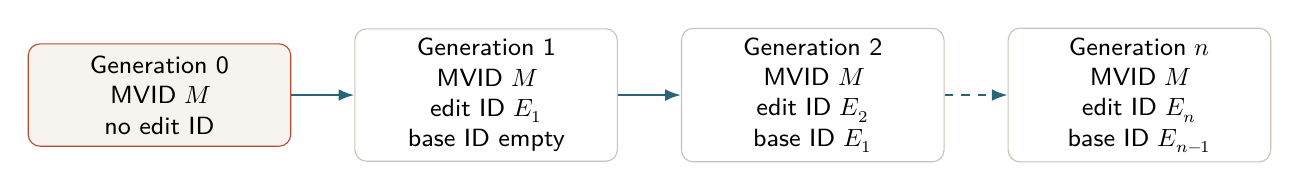
\begin{tikzpicture}[
  gen/.style={draw=PhoenixRule,rounded corners=1.5mm,fill=white,text width=31mm,minimum height=13mm,align=center,font=\small\sffamily},
  base/.style={gen,draw=PhoenixOrange,fill=PhoenixPaper},
  edge/.style={-{Latex[length=2mm]},draw=PhoenixBlue,line width=0.8pt}
]
\node[base] (g0) {Generation 0\\MVID \(M\)\\no edit ID};
\node[gen,right=8mm of g0] (g1) {Generation 1\\MVID \(M\)\\edit ID \(E_1\)\\base ID empty};
\node[gen,right=8mm of g1] (g2) {Generation 2\\MVID \(M\)\\edit ID \(E_2\)\\base ID \(E_1\)};
\node[gen,right=8mm of g2] (gn) {Generation \(n\)\\MVID \(M\)\\edit ID \(E_n\)\\base ID \(E_{n-1}\)};
\draw[edge] (g0) -- (g1);
\draw[edge] (g1) -- (g2);
\draw[edge,dashed] (g2) -- (gn);
\end{tikzpicture}
\caption{Measured Edit-and-Continue lineage relation retained by the E3 contracts.}
\label{fig:enc-lineage}
\end{figure}

E3 stops at physical delta acquisition and lineage. It does not yet project effective logical metadata tables; that is E4's job. This sequencing avoids a dangerous shortcut where a consumer starts using delta rows without a complete and replayable composition model.

\section{Common metadata mistakes to avoid}

\begin{itemize}
  \item Treating MVID alone as complete artifact identity.
  \item Letting a path or simple assembly name decide a join.
  \item Re-resolving a method token during execution after preparation froze a different definition.
  \item Returning the first same-name member instead of counting conflicts.
  \item Calling a partial table scan ``not found.''
  \item Using analysis-runtime reflection for target enum/type facts.
  \item Combining a generation-zero body with generation-aware metadata.
  \item Dropping physical rows after composing an effective view; history is part of replay identity.
\end{itemize}

\begin{sourcebox}
Primary files: \repoPath{Metadata.Abstractions/IMetadataModule.cs}, \repoPath{Metadata.SRM/SrmMetadataModule.cs}, \repoPath{Metadata.SRM/SrmMetadataProjection.cs}, the \repoPath{MetadataAuthority*} and \repoPath{StaticField*Catalog*} families in \repoPath{Product.DumpQuery}, and \repoPath{MetadataEditGenerationContracts.cs}. Pair them with \repoPath{MetadataIdentityTests.cs}, signature projection tests, and the W7/W8 metadata integration suites.
\end{sourcebox}


\chapter{The ClrMD host adapter and physical evidence}
\label{ch:host}

\section{Adapter ownership}

\repoPath{PhoenixInspect.Host.Dump.ClrMD} is the physical boundary between PhoenixInspect contracts and ClrMD/runtime implementation objects. \typeName{ClrmdDumpSession} owns every ClrMD lifetime. No \typeName{DataTarget}, \typeName{ClrRuntime}, \typeName{ClrHeap}, \typeName{ClrType}, or similar adapter object escapes into product or UI layers. Escaping one would leak thread-affinity, lifetime, caching, and version assumptions into code that currently depends only on immutable PhoenixInspect identities.

The session is a large partial class because its surface is grouped by evidence family: arrays, references, frame variables, method/source resolution, static fields, and expression context. The central file owns opening, world identity, module catalogs, memory, and common policy.

\section{Opening a dump}

The open path is deliberately conservative:

\begin{enumerate}
  \item validate and open the dump file under a maximum file-size policy;
  \item keep a read-only stream alive for the session so replacing the path cannot change bytes behind an established identity;
  \item hash the complete dump for snapshot identity;
  \item create the ClrMD data target using an offline component locator rather than ambient machine resolution;
  \item require the admitted runtime shape (currently one CLR runtime for the main walking-skeleton path);
  \item create a counted process-memory reader with the target's pointer width and stable memory-source identity;
  \item enumerate bounded runtime module instances into immutable PhoenixInspect descriptors;
  \item return an exact session or a typed unavailable/unsupported/invalid result.
\end{enumerate}

The dump cache is bounded and selected ClrMD caches are disabled where they could blur counted observation. The adapter is not promising arbitrary cross-version runtime layout support; the tested surface is tied to named fixtures and same-toolchain evidence.

\section{Live attach}

\typeName{AttachToProcess} suspends the target for the lifetime of the session. Disposal detaches and resumes it. The session records process identity and attach time, but explicitly states that its digest is an attach-circumstances identity rather than an immutable content hash.

This lets the same inspection APIs work against dump and live sources while preserving the semantic difference. A host report explains that a live read is repeatable only while this suspended session exists.

\section{Counted raw memory}

\typeName{IProcessMemoryReader} and \typeName{MemoryReadResult} distinguish:

\begin{itemize}
  \item exact read: every requested byte was obtained;
  \item short/partial read: a prefix was obtained and its exact length is known;
  \item unavailable read: no admissible bytes were obtained;
  \item invalid request: range, width, or structural request was malformed.
\end{itemize}

A caller cannot decode an Int32 or pointer unless the required byte width was read exactly. The missing suffix is never zero-filled. Each read is bounded and carries source identity so result provenance can name the physical memory source and address.

\begin{invariantbox}
``Address exists'' and ``value is readable'' are separate facts. A runtime structure can identify a field location while a sparse dump omits the page containing its value. PhoenixInspect retains the exact location evidence and reports the storage read as partial or unavailable.
\end{invariantbox}

\section{Module instances}

A runtime can load logically identical module content into multiple application domains or contexts. The adapter therefore exposes module \emph{instances} with runtime identity, application-domain identity, metadata address/length, layout, and a target-side path hint. Product binding first selects a metadata declaration, then requires exactly one matching runtime module instance under the active contract. Zero matches are unavailable; multiple matches are ambiguous.

Module content identity is computed from counted metadata bytes read from the snapshot, not from the hinted disk path. The hint can seed PDB or assembly candidate discovery, but each candidate must independently reproduce the expected identity.

\section{Heap, roots, and object identity}

The current heap-search surface is deliberately rooted. A bounded strong-handle traversal searches exact ordinal type names and returns retained matches plus traversal counters and caps. This avoids pretending that a filtered or partial heap walk found every object.

An exact result can be converted to a \typeName{DumpObjectBinding}. Static-field evaluation can also promote an exact non-null object reference into a root. In both cases the binding records snapshot, object address/type identity, and provenance describing how the root was selected.

Object addresses are never globally meaningful. The same numeric address in another snapshot does not identify the same object, and the query engine checks this before binding a field.

\section{Instance fields and arrays}

Field lookup combines runtime type information with declared field identity and bounded ancestry traversal. The returned descriptor carries offset/type/declaration facts needed for later reads. A read then validates object/reference shape, computes address geometry under target pointer width, obtains exact bytes or a typed short/unavailable result, and decodes only the admitted value kinds.

Arrays are represented as immutable virtual sequences when their shape and element reads can be established. The expression evaluator can consume those sequences through deterministic operators without copying target objects into the analysis runtime's ordinary collection semantics. Bounds are retained for dimensions, lengths, element reads, and result materialization.

\section{Frames and variables}

A selected frame is named by snapshot-scoped thread and frame ordinals. The adapter intentionally does not publish a fabricated thread count. Probing an ordinal beyond the end and probing a live thread with no managed frame can produce the same typed unavailable observation; the inspection service explains this ambiguity instead of inferring which one occurred.

Exact managed frames retain runtime thread identity, module/method tokens, stack/instruction context, and module content identity. Variable projection decodes parameters and local slots where the dump/runtime/PDB evidence permits. Optimized code can legitimately make source locals unavailable or remapped; separate optimized-context fixtures preserve those limits as expected behavior.

\section{Method bodies and execution resolver}

\typeName{ClrmdDumpExecutionResolver} joins runtime method observations, counted module metadata, and the reusable SRM projection into execution-core definitions. It is responsible for the host-specific part of W3/W4 admission: locating the exact runtime/module method, reading the admitted body bytes, resolving same-module operands, and exposing structured failures.

The execution core never sees ClrMD methods. It sees \typeName{ResolvedMethodDefinition}, \typeName{ResolvedField}, and structural handles. This keeps graph planning deterministic and testable with synthetic resolvers.

\section{Static fields}

Static storage is one of the adapter's densest areas because CLR storage varies by field kind, declaring type, app domain, thread/context, nullable layout, and runtime implementation. The W7/W8 contracts split the path into:

\begin{enumerate}
  \item metadata declaration identity;
  \item runtime module/type/field mapping;
  \item decoder expectation;
  \item storage-base/location evidence;
  \item counted raw read;
  \item terminal value observation;
  \item optional object-reference and assignability proof.
\end{enumerate}

A nullable Int32, for example, requires an independently projected runtime layout for its \codeinline{HasValue} and \codeinline{Value} children. The product composes metadata child roles with the runtime layout and stops if they conflict.

\section{Portable PDB and source location}

The adapter validates PDB candidates against module debug identity and returns a source \emph{location}: document identity, checksum algorithm/checksum, line span, and artifact identity. It does not read and display the local source file. That final trust decision belongs to the inspection layer because it may involve local files, embedded source, explicit SourceLink network capability, or decompilation presentation.

This separation allows headless product tests to prove binding/context facts without granting arbitrary file or network access.

\section{Session-level bounds}

Representative caps include:

\begin{itemize}
  \item dump file size up to 8 GiB;
  \item bounded cache memory;
  \item 4,096 module instances and 4,096 instance-field traversal units;
  \item 100,000 handle scans and 4,096 retained handle matches;
  \item 10,000 method scans for relevant host operations;
  \item 1,048,576 observed string characters at the broad adapter boundary, with tighter product-specific limits;
  \item bounded frame/thread traversal, PDB candidates, artifact bytes, and raw read widths.
\end{itemize}

A product layer can impose a stricter bound than the adapter. Both can appear in evidence when both were reached; configured but irrelevant caps do not.

\section{The dedicated adapter thread}

ClrMD's underlying reader is not treated as concurrently safe. \typeName{DumpSessionHost} in the inspection project owns one long-lived worker thread and a \typeName{BlockingCollection<Action>}. Every session open, close, attach, and query runs on that thread; results are marshalled back through \typeName{TaskCompletionSource<T>} with asynchronous continuations.

\begin{figure}[htbp]
\centering
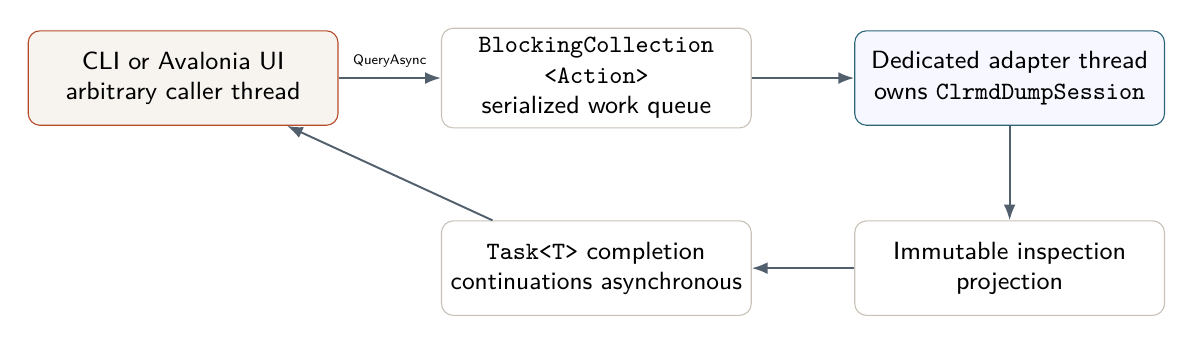
\begin{tikzpicture}[
  box/.style={draw=PhoenixRule,rounded corners=1.5mm,fill=white,text width=37mm,minimum height=12mm,align=center,font=\small\sffamily},
  edge/.style={-{Latex[length=2mm]},draw=PhoenixMuted,line width=0.7pt}
]
\node[box,fill=PhoenixPaper,draw=PhoenixOrange] (ui) {CLI or Avalonia UI\\arbitrary caller thread};
\node[box,right=13mm of ui] (queue) {\texttt{BlockingCollection}\\\texttt{<Action>}\\serialized work queue};
\node[box,right=13mm of queue,fill=blue!3,draw=PhoenixBlue] (worker) {Dedicated adapter thread\\owns \typeName{ClrmdDumpSession}};
\node[box,below=12mm of worker] (projection) {Immutable inspection\\projection};
\node[box,left=13mm of projection] (task) {\typeName{Task<T>} completion\\continuations asynchronous};
\draw[edge] (ui) -- node[above=1mm,font=\tiny\sffamily,fill=white,inner sep=0.7pt]{QueryAsync} (queue);
\draw[edge] (queue) -- (worker);
\draw[edge] (worker) -- (projection);
\draw[edge] (projection) -- (task);
\draw[edge] (task) -- (ui);
\end{tikzpicture}
\caption{Host-side serialization of every ClrMD operation. Only immutable PhoenixInspect projections return to UI code.}
\label{fig:adapter-thread}
\end{figure}

Opening another world disposes the prior session first. This prevents a rendered result from mixing module lists or object roots from two snapshots. Disposing the host closes the session on the worker thread, completes the queue, and joins the worker.

\section{Where adapter bugs usually hide}

\begin{itemize}
  \item a ClrMD object escaped its session or thread;
  \item a target-side path hint was accidentally treated as identity;
  \item a short read was decoded as a full scalar;
  \item a runtime module instance join ignored app-domain/runtime identity;
  \item a bound was reached but not carried into the product result;
  \item a cached runtime observation came from a different world;
  \item a runtime layout assumption was not pinned to tested descriptor/toolchain evidence;
  \item a filtered dump was treated as ``zero'' rather than unavailable.
\end{itemize}

\begin{sourcebox}
Begin with \repoPath{ClrmdDumpSession.cs}, \repoPath{ClrmdProcessMemoryReader.cs}, \repoPath{ClrmdModuleInfo.cs}, and \repoPath{SnapshotIdentity.cs}; then follow the relevant partial file for arrays, references, frames, source, or static fields. For execution, read \repoPath{ClrmdDumpExecutionResolver.cs}. For threading, read \repoPath{Inspection/Infrastructure/DumpSessionHost.cs}. Real-dump behavior is concentrated in \repoPath{PhoenixInspect.IntegrationTests}.
\end{sourcebox}

\chapter{Parsing, binding, rooted queries, and expression evaluation}
\label{ch:query}

\section{Why \texttt{Product.DumpQuery} is larger than its name}

The project began with a narrow root-field query and now contains several cooperating expression subsystems:

\begin{itemize}
  \item the sole pinned Roslyn C\# expression parser and versioned admission profiles;
  \item the original W2 rooted field query and immutable plan;
  \item fixed-depth and later arbitrary-depth admitted member chains;
  \item W7/W8 static-field syntax, metadata binding, runtime mapping, and storage reads;
  \item a large deterministic expression evaluator;
  \item type/enum/array/sequence/temporal/query/anonymous-object value models;
  \item source-anchored metadata authority and edit-generation contracts.
\end{itemize}

Its unifying principle is read-only derived truth. Even when it evaluates rich syntax, it either folds deterministic values or composes observations from the snapshot. It does not interpret arbitrary user methods; that transition belongs to \repoPath{Product.DumpDebugging}.

\section{One pinned parser}

\typeName{CSharpExpressionFrontEnd} and \typeName{DumpQueryParser} centralize parsing under Roslyn 5.3.0, C\# 14, and a named project profile. The parser accepts a complete expression with full-text consumption and rejects directives, disabled text, skipped tokens, missing tokens, overlong input, excessive syntax depth, or excessive node/token count.

Representative bounds include:

\begin{itemize}
  \item 512 expression characters;
  \item 256 syntax nodes plus tokens;
  \item syntax depth 64;
  \item identifier length 64;
  \item bounded string-literal length.
\end{itemize}

The front end distinguishes invalid C\# from valid C\# outside the current project-owned profile. This is essential for forward evolution: adding an admitted construct changes the profile version and contract, not the meaning of ``valid syntax.''

\section{Versioned expression descriptors}

After Roslyn parsing, the product converts syntax to immutable project-owned descriptors. Downstream code does not retain Roslyn nodes as semantic identities. Profiles include historical frozen W2/W5 forms, fixed-depth member-chain admission, and the current opt-in member-chain V2 surface.

The descriptor records normalized structural information but preserves enough raw/request identity to produce stable policy provenance. Selection occurs once. Later stages use the descriptor and selected plan rather than reparsing or rediscovering candidate shapes.

\begin{invariantbox}
Roslyn answers ``what syntax did the user write?'' PhoenixInspect answers ``which subset and semantic profile is admitted?'' The second question must never be delegated to whatever Roslyn happens to support in a future package version.
\end{invariantbox}

\section{The W2 rooted query}

\typeName{DumpQueryEngine} remains a useful miniature of the whole architecture. Its original grammar is intentionally tiny: one exact root identifier, one instance-field name, and optional null/Int32/string coalescing.

\subsection{Preparation}

Preparation performs:

\begin{enumerate}
  \item syntax classification under parser bounds;
  \item validation of upstream root-binding bounds;
  \item snapshot identity comparison;
  \item root-binding status check;
  \item one bounded runtime field selection;
  \item field-kind classification and coalesce compatibility;
  \item construction of an immutable \typeName{DumpQueryPlan} carrying the selected root, field descriptor, parser/adapter bounds, and provenance identity.
\end{enumerate}

A search-backed root retains the exact type predicate, adapter status, traversal counters, and caps. This means two roots at the same address selected under different evidence do not automatically yield the same plan identity.

\subsection{Evaluation}

Evaluation consumes the frozen field descriptor. It does not call member lookup again. It reads the selected field under the exact snapshot and decodes according to the plan's field kind. Exact null, exact Int32, bounded string, partial bytes, and unavailable bytes remain distinct.

This separation is small enough to study but general enough to serve as a pattern for later member chains and methods.

\section{Member chains}

The member-chain engine extends the same discipline across multiple hops. The syntax descriptor determines the exact chain, conditional-access boundaries, and fallback. Each hop:

\begin{enumerate}
  \item starts from an exact object or nullable/reference state produced by the prior hop;
  \item selects a declared runtime field once;
  \item records its field identity and evidence;
  \item reads and decodes the value under bounds;
  \item either continues with an object binding, returns a terminal value, applies conditional-null semantics, or stops with a typed disposition.
\end{enumerate}

An arbitrary-depth user expression is therefore still a finite bounded operation: expression length and node count bound the number of admitted segments; each field/ancestry/read operation has its own cap; result materialization has another cap.

Conditional access is semantic, not an exception suppressor. It only bypasses the suffix when the receiver is an exact null under the admitted nullable/reference semantics. An unavailable receiver does not become null.

\section{Static-field expression pipeline}

\typeName{StaticFieldExpressionEvaluator} runs a larger parse/bind/map/read/compose pipeline. Its high-level stages are:

\begin{longtable}{L{42mm}L{107mm}}
\toprule
\textbf{Stage} & \textbf{What is established} \\
\midrule
\endfirsthead
\toprule
\textbf{Stage} & \textbf{What is established} \\
\midrule
\endhead
Syntax & Exactly one accepted static-field descriptor and candidate-shape set. \\
Symbol binding & One metadata declaration, or a typed absent/ambiguous/context-required/invalid stop. \\
Runtime declaration & Exactly one runtime module/type/field mapping corresponding to that metadata declaration. \\
Nullable layout & Exact runtime child-role geometry when the declared type is nullable Int32. \\
Storage request & A physical read request whose decoder and storage identity agree with metadata/runtime evidence. \\
Storage observation & Counted bytes and terminal scalar/reference/null outcome. \\
Assignability & For non-null references, proof that the runtime object is admissible for the declared field type. \\
Suffix evaluation & Optional direct member/chain/fallback evaluation over an exact object-reference result. \\
Composition & One replayable result retaining exact prefixes, stops, bounds, observations, and optional promotable root. \\
\bottomrule
\end{longtable}

\subsection{Lazy context acquisition}

The overload taking a selected-frame selector and PDB candidates does not immediately inspect the frame. It first tries context-independent fully qualified binding. Only when a bare/source-like spelling genuinely needs imports, namespace, or aliases does it acquire frame/PDB context.

This avoids three problems:

\begin{itemize}
  \item a fully qualified expression should not fail because an unrelated frame is unavailable;
  \item exact context-independent replay should not depend on a PDB candidate set it never consulted;
  \item the adapter should not perform expensive or capability-sensitive work speculatively.
\end{itemize}

A descriptor containing a global qualifier also remains context-independent by construction.

\subsection{Metadata-to-runtime join}

After exact symbol binding, the evaluator matches the selected declaration's module identity against runtime module instances. Exactly one match is required. It then calls the session's runtime-declaration mapper using definition tokens, declaring-type identity, field name, and expected decoder. These redundant-looking inputs cross-check one another; they are not merely lookup conveniences.

Nullable layout and reference assignability are composed in separate steps so a failure can name the exact unsupported/conflicting boundary.

\subsection{Root promotion}

An exact non-null object-reference static field can produce a \typeName{DumpObjectBinding} with provenance identifying the static expression. The inspection layer exposes this as a promotable root. This is necessary because an object can be reachable from a static field without appearing in the bounded strong-handle catalog.

\section{The deterministic expression evaluator}

\typeName{ExpressionEvaluator} is split across partial files by semantic family: numeric, syntax, arrays, sequences, queries, lambdas, temporal values, enums, types, tuples, anonymous objects, and supporting value models. It is best understood as a pure interpreter for a closed expression language, not as ``compile and invoke C\#.''

Its top-level status is one of:

\begin{description}[style=nextline]
  \item[NotFolded] The expression should fall through to another product pipeline unchanged.
  \item[Exact] A deterministic value was produced under the admitted constant/profile semantics.
  \item[Invalid] The expression selected this pipeline but violated syntax, typing, bounds, or deterministic operation rules.
\end{description}

A bare dump field or member chain deliberately remains outside the folding pre-stage so its existing evidence report and replay digest stay byte-identical. A composed expression such as \codeinline{root.QueueDepth * 2 + 1} enters the expression evaluator, which calls the frozen root pipeline for the operand and consumes its exact value.

\section{Value families}

The evaluator's result model includes Int32, general numeric values, strings/chars/booleans/null, enums, sequences, temporal values, deterministic BCL values, type references, tuples, and anonymous objects. The implementation aims to reproduce C\# and selected BCL semantics rather than invent convenient approximations.

\subsection{Numeric semantics}

The supported tower includes fixed-size integral types, \typeName{Int128}/\typeName{UInt128}, \typeName{BigInteger}, IEEE-754 \typeName{float}/\typeName{double}, and exact-scale \typeName{decimal}. Promotions, checked/unchecked contexts, conversions, comparisons, and formatting are explicit. Host culture is not consulted.

\subsection{Sequences and LINQ}

Array initializers, collection expressions with spreads, dump-backed arrays, and folded sequences share a virtual sequence model. Deterministic \typeName{Enumerable} operations and expression lambdas execute within bounded evaluator semantics. Operations that mutate or rely on ambient comparer/culture/time state are rejected or modelled only under an explicit deterministic contract.

\subsection{Temporal and BCL values}

\typeName{DateTime}, \typeName{DateTimeOffset}, \typeName{TimeSpan}, \typeName{DateOnly}, and \typeName{TimeOnly} are admitted for deterministic construction, ticks, arithmetic, comparison, and invariant formatting. \codeinline{Now}, local-time conversion, and culture-dependent parsing are typed stops. Likewise, \typeName{Guid} and \typeName{Version} have fixed-grammar construction/parsing and comparison; \codeinline{Guid.NewGuid()} is not evidence and is rejected.

\subsection{Enums and types}

Enum shape is read from the captured module's metadata. Casts, bitwise flags, \codeinline{HasFlag}, formatting, and selected \typeName{System.Enum} operations use that target authority. \codeinline{typeof} and deterministic \typeName{System.Type} operations operate over structural type values, including arrays, generic definitions/instantiations, assignability, variance, and declared base/interface relationships where exact metadata support exists.

\subsection{Queries and modern C\# forms}

Query syntax is translated according to C\# rules onto the admitted folded operator surface. Anonymous objects retain projected names, structural equality, invariant formatting, and expandable members. Interpolated strings, selected patterns and switch expressions, \codeinline{nameof}, \codeinline{default(T)}, \codeinline{sizeof(T)}, and checked wrappers are handled within the same deterministic restrictions.

\section{Canonical identity and display expansion}

The constant outcome has its own domain/versioned canonical digest. Expandable children for arrays, tuples, and anonymous objects are a presentation projection and do not perturb the value digest. This lets a host materialize a bounded child list without changing the identity of the parent answer.

\section{Expression routing above the project}

The shared inspection layer routes a Watch expression lexically:

\begin{itemize}
  \item if an adopted root exists and the root identifier appears as a standalone token, use the root-relative product path;
  \item otherwise use the static-field path.
\end{itemize}

The rule is deliberately total and non-parsing. The root-relative path can also resolve context-free static operands, so a mixed expression can route there and combine both. An occurrence inside an interpolated string still routes to the root path; at worst, the richer resolver answers an expression the static path could also answer.

\section{Failure interpretation}

When debugging an expression result, identify the last completed stage:

\begin{enumerate}
  \item Roslyn syntax;
  \item project profile admission;
  \item metadata binding;
  \item runtime declaration mapping;
  \item physical storage or object hop;
  \item deterministic value composition;
  \item method-path handoff, if any.
\end{enumerate}

A failure at stage 3 should not be ``fixed'' by making storage lookup more permissive. The typed result and retained exact prefix exist precisely to prevent such cross-layer guessing.

\begin{sourcebox}
Core reading order: \repoPath{DumpQueryParser.cs}; \repoPath{DumpQueryEngine.cs} and \repoPath{DumpQueryPlan.cs}; member-chain parser/plan/engine files; \repoPath{StaticFieldExpressionEvaluator.cs}; then the partial \repoPath{ExpressionEvaluator.*.cs} families. Tests are organized similarly: parser/plan tests, \repoPath{ConstantExpression*Tests.cs}, and real-dump member/static-field suites.
\end{sourcebox}


\chapter{Counterfactual method evaluation}
\label{ch:counterfactual}

\section{The product-level handoff}

\repoPath{PhoenixInspect.Product.DumpDebugging} is where dump evidence becomes a counterfactual machine input. It owns expression classification, method acquisition, virtual memory import, request/preparation contracts, execution, and result projection. It references the query product because field/member/static operands can be part of the expression path and because their exact evidence is reused rather than reimplemented.

\typeName{DumpExpressionEvaluator} returns a strict union. Representative alternatives include:

\begin{itemize}
  \item derived query result;
  \item counterfactual execution result;
  \item classification failure;
  \item dump acquisition failure;
  \item counterfactual preparation failure.
\end{itemize}

The facade does not force every route into one fake lattice. A W2 field query and a W4 method execution retain their native contracts and semantic modes.

\section{Classification before evidence}

Expression classification occurs before touching dump evidence. Rejected syntax cannot enumerate modules, read fields, or query resolvers. This capability ordering is tested and matters for both performance and replay: a syntax-only rejection should not depend on which dump happened to be open.

For a method path, classification yields a structural descriptor that drives acquisition. The product then resolves the rooted receiver, method declaration, arguments, field observations, and policy into a preparation candidate.

\section{Counterfactual request identity}

\typeName{CounterfactualMethodRequest} freezes the public semantic request:

\begin{itemize}
  \item evidence source and snapshot/module identity;
  \item root-selection identity and root evidence digest;
  \item root method and receiver/argument evidence;
  \item policy ID/version and instruction/depth/traversal limits;
  \item model catalog ID/version and optional required modeled target;
  \item explicit assumptions.
\end{itemize}

The request is validated for mutual compatibility before graph planning. A malformed candidate becomes a stable value-free failure, not an exception-controlled result.

\section{Preparation candidate and private runtime bundle}

The preparation candidate additionally carries capabilities and data that should not become public request identity: resolver, value domain, memory model, initial persistent memory, materialized receiver/arguments, field observations, and optional model registry.

After validation and graph preparation, these are sealed into a private runtime bundle. The public plan exposes canonical facts; the executable capabilities remain private. This protects replay from callers swapping a resolver or memory model after a plan's digest has been computed.

\section{Private plan issuance}

Each \typeName{CounterfactualMethodRunner<TMemory>} creates a private issuer object. Successful plans are stamped with that issuer. \typeName{Run} checks plan authority before observing cancellation, reading public plan fields, or touching private capabilities. A null or foreign plan returns a fixed identity-free facade rejection.

This is stronger than a type check. A plan issued by another runner instance is structurally plausible but not authorized to use this runner's retained runtime bundle. The design resembles an object-capability boundary inside the process.

\begin{figure}[htbp]
\centering
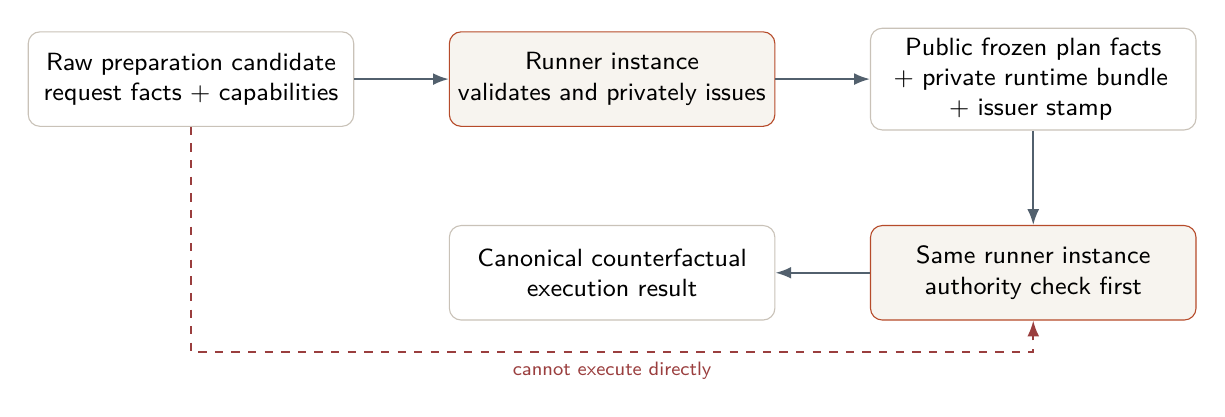
\begin{tikzpicture}[
  box/.style={draw=PhoenixRule,rounded corners=1.5mm,fill=white,text width=39mm,minimum height=12mm,align=center,font=\small\sffamily},
  auth/.style={box,draw=PhoenixOrange,fill=PhoenixPaper},
  edge/.style={-{Latex[length=2mm]},draw=PhoenixMuted,line width=0.7pt}
]
\node[box] (candidate) {Raw preparation candidate\\request facts + capabilities};
\node[auth,right=12mm of candidate] (prepare) {Runner instance\\validates and privately issues};
\node[box,right=12mm of prepare] (plan) {Public frozen plan facts\\+ private runtime bundle\\+ issuer stamp};
\node[auth,below=12mm of plan] (run) {Same runner instance\\authority check first};
\node[box,left=12mm of run] (result) {Canonical counterfactual\\execution result};
\draw[edge] (candidate) -- (prepare);
\draw[edge] (prepare) -- (plan);
\draw[edge] (plan) -- (run);
\draw[edge] (run) -- (result);
\coordinate (rejectlane) at ([yshift=-4mm]result.south);
\draw[edge,dashed,draw=PhoenixRed]
  (candidate.south) -- (candidate.south |- rejectlane)
  -- node[below,font=\scriptsize\sffamily,text=PhoenixRed]{cannot execute directly}
  (run.south |- rejectlane) -- (run.south);
\end{tikzpicture}
\caption{Private issuance prevents a caller from assembling an executable-looking plan from public data.}
\label{fig:private-plan}
\end{figure}

\section{Preparation sequence}

\typeName{Prepare} performs, in order:

\begin{enumerate}
  \item null/raw candidate validation;
  \item canonical request creation;
  \item capability/binding compatibility checks;
  \item one graph-planning attempt, with optional required pure model;
  \item planner success/failure coherence validation;
  \item logical-depth sufficiency check;
  \item root signature versus receiver/argument compatibility;
  \item field-observation completeness/order/receiver validation;
  \item provenance-domain argument materialization;
  \item private plan issuance.
\end{enumerate}

Every ordinary malformed-input exception is normalized into a stable result. Catastrophic process exceptions are not swallowed.

\section{Recording memory}

Execution wraps the underlying memory model in \typeName{CounterfactualRecordingMemoryModel}. The wrapper knows the predeclared field observations and the rooted receiver. It rejects an unexpected load rather than querying ambient dump state during execution. Reached load ordinals and observations are recorded in exact dynamic order.

This closes a subtle replay hole. A frozen graph can prove which fields are syntactically reachable, but branch/model behavior determines which loads actually occur. The result should cite reached evidence, while still ensuring no undeclared load can escape the plan.

\section{Rejecting execution-time resolution}

The machine is created with \typeName{RejectingExecutionResolver.Instance}. Any accidental resolution attempt inside the execution loop is therefore a hard capability failure. All definitions and call targets must come from the frozen graph.

This is one of the best architectural tests in the repository: rather than relying on code review to notice a resolver call, the product supplies a resolver whose only valid behavior is rejection.

\section{The run loop}

Before stepping, the runner:

\begin{itemize}
  \item calculates a finite dynamic instruction cost from the acyclic graph;
  \item creates provenance domain, recording memory, machine, and operational budget;
  \item activates the prepared graph;
  \item validates the exact single-root activation state;
  \item initializes call trace and event builders;
  \item derives a maximum step-request count including the terminal idempotence check.
\end{itemize}

Each iteration then:

\begin{enumerate}
  \item validates the state envelope;
  \item observes cancellation only at a ready boundary;
  \item enforces the graph-derived step-request maximum;
  \item calls \typeName{StepOne};
  \item verifies the machine-issued transition stamp;
  \item validates budget, event, frame, model, memory, and terminal-union deltas;
  \item appends dynamic calls/events;
  \item dispatches on \status{Ready}, \status{Completed}, \status{BudgetExhausted}, \status{Blocked}, \status{InvalidProgram}, or target exception.
\end{enumerate}

A capability exception becomes a stable blocked/invalid result depending on where it occurred. An impossible transition becomes a replay-invalid result with a diagnostic naming the violated contract.

\section{Completion and result projection}

A normal completion must leave an empty call stack, one root return value, no terminal target exception, and the same read-only initial memory identity. The mandatory terminal re-step must be idempotent. The runner then projects:

\begin{itemize}
  \item semantic mode \truthmode{CounterfactualExecution};
  \item completion/completeness/evidence/effects axes;
  \item typed return or execution-prefix value;
  \item instruction/depth/lineage bound status and high-water marks;
  \item reached field observations and load ordinals;
  \item model attempts and counts;
  \item dynamic call trace and debug events;
  \item stable diagnostics and canonical replay identity.
\end{itemize}

Effect status reflects virtual or modeled behavior, never mutation of the captured process.

\section{Why the runner revalidates its own machine}

At first glance, transition validation appears redundant: the machine and runner live in the same repository. It serves several purposes:

\begin{itemize}
  \item the generic machine consumes external domain/memory/model capabilities whose implementations can be buggy;
  \item product-level canonical results need stronger invariants than a low-level stepper's convenience API;
  \item tests can inject hostile or incoherent capabilities and prove prefix-free failure;
  \item future machine changes cannot silently alter event/budget/frame contracts without breaking product tests;
  \item replay identity is protected from malformed internal states rather than trusting them by convention.
\end{itemize}

The runner is thus a certification boundary, not a thin loop wrapper.

\section{Modeled calls}

A pure model has a versioned catalog identity and explicit attempt result. The operational envelope retains every attempt, whether it completed a transfer or failed. A successful model consumes one instruction transfer under the closed contract, advances logical depth, may avoid an interpreted frame, and contributes transformation provenance.

A required model target is part of the request. The planner cannot silently fall back to interpretation if the required model is absent, nor can an interpreted-only policy consult a model registry.

\section{Counterfactual memory and assumptions}

The method path imports exact root and field observations into virtual memory. Assumptions are explicit request fields, not ambient facts. The product can therefore distinguish:

\begin{itemize}
  \item an exact captured receiver field;
  \item a virtual value introduced under a named assumption;
  \item a modeled helper result;
  \item an unknown caused by unsupported or missing evidence.
\end{itemize}

That distinction will be necessary for future virtual stepping or abstract analysis, where the virtual world diverges further from the dump.

\begin{sourcebox}
Read \repoPath{DumpExpressionEvaluator.cs}, the \repoPath{CounterfactualMethodRequest*}, \repoPath{CounterfactualMethodPreparation*}, \repoPath{CounterfactualMethodPlan*}, \repoPath{CounterfactualRecordingMemoryModel.cs}, and \repoPath{CounterfactualMethodRunner.cs}. The result/canonical-codec files explain final replay shape. The corresponding \repoPath{Counterfactual*Tests.cs} and \repoPath{PreparedGraph*Tests.cs} cover hostile and edge-case capabilities.
\end{sourcebox}

\chapter{Inspection services and the three hosts}
\label{ch:hosts}

\section{A deliberately thin presentation layer}

\repoPath{PhoenixInspect.Inspection} is the shared host-facing layer. Both the console and Avalonia applications reference it; neither references the product internals directly. Its job is to:

\begin{itemize}
  \item own one serialized dump/live session;
  \item invoke adapter and product entry points on the correct thread;
  \item project outcomes into immutable display models;
  \item format stable facts without changing their meaning;
  \item maintain host-facing root/frame/PDB context;
  \item provide completion, process discovery, source navigation, and expansion services.
\end{itemize}

Its XML comments repeatedly state that it does not widen or reinterpret adapter/product outcomes. Statuses, issues, counters, bounds, and digests are carried through. This is the architectural reason the CLI and desktop produce semantically comparable answers.

\section{Display models}

The models project defines value-like records for snapshot properties, module rows, frame variables, call-stack nodes, heap matches, diagnostics, evidence facts, source lines, and evaluation reports. They are deliberately detached from ClrMD lifetimes. A UI may cache or bind them after the adapter operation completes.

\typeName{EvaluationReport} is not a replacement result contract. It is a host-oriented projection containing the original status vocabulary, path/stage description, rendered value/type, evidence facts, diagnostics, reached bounds, digest, optional expandable children, and optional promotable root.

\section{\typeName{DumpInspectionService}}

This service handles non-expression inspection:

\begin{itemize}
  \item snapshot/live-session overview and declared-bound facts;
  \item module-instance listing and counted metadata identity;
  \item bounded thread probing and frame loading;
  \item parameters/locals projection;
  \item heap-object search;
  \item source-selection inputs and related rows.
\end{itemize}

A particularly good example is call-stack probing. The service does not infer a thread count the adapter does not provide. It returns nodes for ordinals with an exact managed frame and an explanatory note for indistinguishable unavailable cases. Presentation text is thus derived from the adapter's epistemic boundary rather than from debugger convention.

\section{\typeName{ExpressionEvaluationService}}

The expression service presents two host-facing paths:

\begin{description}[style=nextline]
  \item[Static field] Fully qualified or contextual static expressions, with the folding pre-stage and optional root promotion.
  \item[Root relative] Member/method/composed expressions against an adopted root under host-friendly policy options.
\end{description}

Host options are mapped to product contracts: modeled versus interpreted methods, member-chain profile, instruction limit, logical-depth limit, and traversal limit. The service clamps values to product maxima so a front end cannot accidentally bypass hard policy.

Watch routing uses the standalone-token scan described in Chapter~\ref{ch:query}. The report always names the path that answered. This makes a transcript auditable even if the same text could in principle be resolved by more than one subsystem.

\section{Completion}

Completion candidates are evidence-derived and profile-aware. The completion service combines:

\begin{itemize}
  \item C\# keywords and modeled deterministic types/members;
  \item root fields from the adopted object's exact runtime type;
  \item namespaces, types, and static fields from dump-module metadata;
  \item contextual/import information when exact frame/PDB context is active.
\end{itemize}

The intended invariant is that completion should not suggest a name the evaluator's own current profile cannot answer. Candidate enumeration is bounded and carries session state so a stale drop-down does not become authority after root/context changes.

\section{Source navigation}

\typeName{SourceNavigationService} deliberately separates line mapping from content trust. The adapter establishes which document and span the matching PDB recorded. The inspection service then tries content sources in an evidence-ranked order:

\begin{enumerate}
  \item local file at the recorded path, only if its bytes reproduce the PDB document checksum;
  \item embedded source inside the identity-matching Portable PDB;
  \item SourceLink content, only when the host explicitly enables download, the URL is HTTPS, the byte cap is respected, and the downloaded bytes reproduce the PDB checksum;
  \item C\# decompiled from an on-disk assembly whose complete metadata identity matches the dump module, explicitly labelled as reconstruction;
  \item otherwise a typed unresolved source view.
\end{enumerate}

\begin{figure}[htbp]
\centering
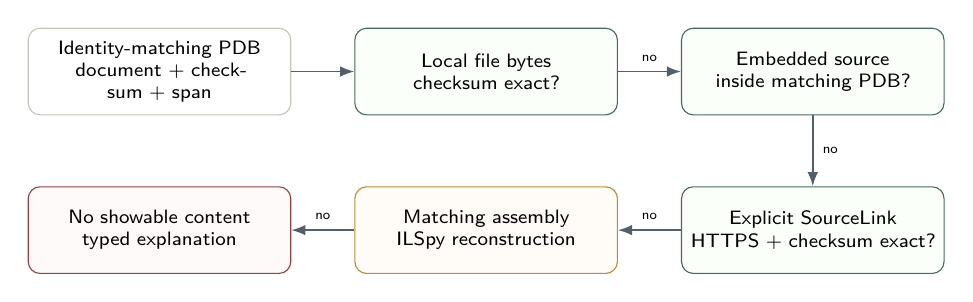
\begin{tikzpicture}[
  box/.style={draw=PhoenixRule,rounded corners=1.5mm,fill=white,text width=31mm,minimum height=11mm,align=center,font=\scriptsize\sffamily},
  good/.style={box,draw=PhoenixGreen,fill=green!2},
  fallback/.style={box,draw=PhoenixGold,fill=orange!3},
  stop/.style={box,draw=PhoenixRed,fill=red!2},
  edge/.style={-{Latex[length=1.8mm]},draw=PhoenixMuted,line width=0.6pt}
]
\node[box] (loc) {Identity-matching PDB\\document + checksum + span};
\node[good,right=8mm of loc] (local) {Local file bytes\\checksum exact?};
\node[good,right=8mm of local] (embedded) {Embedded source\\inside matching PDB?};
\node[good,below=9mm of embedded] (sl) {Explicit SourceLink\\HTTPS + checksum exact?};
\node[fallback,left=8mm of sl] (decomp) {Matching assembly\\ILSpy reconstruction};
\node[stop,left=8mm of decomp] (none) {No showable content\\typed explanation};
\draw[edge] (loc) -- (local);
\draw[edge] (local) -- node[above,font=\tiny\sffamily]{no} (embedded);
\draw[edge] (embedded) -- node[right,font=\tiny\sffamily]{no} (sl);
\draw[edge] (sl) -- node[above,font=\tiny\sffamily]{no} (decomp);
\draw[edge] (decomp) -- node[above,font=\tiny\sffamily]{no} (none);
\end{tikzpicture}
\caption{Source content is shown only through a proved identity/checksum path; decompiled C\# is a separately labelled reconstruction.}
\label{fig:source-fallback}
\end{figure}

The service caps source files at 10 MiB and PDB candidates at 64. Unknown checksum algorithms do not justify a false exact claim. Embedded source can still be shown as artifact-contained evidence with a precise label when no supported checksum algorithm is available, provided the matching PDB itself is authoritative.

\section{Process discovery}

The desktop's Processes pane uses a bounded discovery service to identify likely managed processes and explain the recognition evidence. Discovery does not attach. The user-selected process is then passed to the same session host that the CLI uses, and the attach result still must be exact.

\section{The console host}

\repoPath{PhoenixInspect.Cli} is a full scriptable inspection shell rather than a thin one-command wrapper.

\subsection{Entry and exit codes}

\typeName{Program.Main} supports dump capture, dump open, live attach, scripted commands, repeated evaluations, and an interactive prompt. Exit codes distinguish success, usage error, world-open failure, and command failure. UTF-8 output is selected explicitly.

A session begins by opening/attaching through \typeName{DumpSessionHost}, printing the overview, then running either the scripted sequence or interactive loop. The final summary reports total expressions and the count that were not exact or exhaustively absent. Its wording deliberately describes non-exact results as evidence limits rather than failures to ``try harder.''

\subsection{Session commands}

\typeName{InspectionSession} maintains explicit state:

\begin{itemize}
  \item adopted root and root identifier;
  \item selected frame for name context;
  \item offered Portable-PDB candidates;
  \item latest heap search and module list;
  \item verbose-evidence setting and evaluation counts.
\end{itemize}

Commands include overview/status, modules and module metadata, threads/frames, context selection by ordinal or method name, PDB candidate management/auto-discovery, bounded object search, root adoption from search or static expression, root renaming, evaluation, and exit. A bare line not recognized as a command is evaluated as an expression.

The \codeinline{status} command makes every evidence input visible. This is important for scripted transcripts: a reader can reconstruct why \codeinline{ServiceState.Count} bound contextually in one step and required qualification in another.

A command-level exception is rendered and returns a failed command outcome without destroying the open session. Ordinary product non-exact results are not exceptions and do not fail a script merely because they are partial or unsupported.

\section{The desktop host}

\repoPath{PhoenixInspect.Desktop} uses Avalonia, Dock, AvaloniaEdit, and ProDataGrid to present a debugger-style workspace. The source tree separates:

\begin{itemize}
  \item \repoPath{ViewModels/}: main window, session overview, processes, modules, threads, call stacks, locals, heap objects, Evaluate, Watch, and Immediate;
  \item \repoPath{Views/}: pane XAML and small view-specific interaction code;
  \item \repoPath{Docking/}: dock factory and pane models;
  \item \repoPath{Infrastructure/} and converters: UI-only support;
  \item application resources/themes in \repoPath{App.axaml}.
\end{itemize}

The default layout resembles a debugger: navigation/inspection panes, central documents, evidence/result pane, and bottom-band evaluation/call-stack tools. Docking is a presentation concern. View models call the same inspection services as the CLI.

\subsection{Watch}

Watch rows are editable. The trailing row creates a new watch; clearing a row deletes it. Rows re-evaluate when root or frame context changes. Compound values expose bounded child rows from the report's expansion projection. Each row retains its own status and evidence report rather than sharing a global ``last error.''

\subsection{Immediate}

The Immediate pane is a prompt/transcript over the same routed evaluator. History navigation and completion are UI state; expression semantics are not reimplemented. Results are rendered with C\#-like syntax colouring and trailing status comments, and explained stops are comments rather than bare exception text.

\subsection{Source documents}

Selecting a frame can open a verified source or reconstructed decompilation document. The document title and summary state which evidence path produced it. This avoids a common debugger UI problem where a stale local source file is displayed with authoritative highlighting.

\section{The headless reference consumer}

\repoPath{PhoenixInspect.Headless.ReferenceConsumer} is both a sample client of the public APIs and an executable conformance/corpus host. Its large portfolio runners predeclare scenarios, invoke exact public entry points, render stable reports, compare canonical digests/goldens, and prove that useful analysis does not depend on desktop types.

This project is strategically important:

\begin{itemize}
  \item it catches accidental internal-only dependencies in public contracts;
  \item it supplies a deterministic hosted CI workflow;
  \item it records meaningful synthetic incidents and counterfactual variants;
  \item it provides closure evidence for milestone claims;
  \item it demonstrates how another host could integrate the libraries without copying UI code.
\end{itemize}

\section{Presentation-layer anti-patterns}

\begin{itemize}
  \item Calling ClrMD directly from a view model or CLI command.
  \item Rebinding or reparsing an expression to obtain nicer display text.
  \item Treating \status{Partial} as a red exception and \status{Absent} as an empty string.
  \item Caching a root/frame across session replacement without snapshot identity.
  \item Showing a local source file before checksum verification.
  \item Inventing a UI-only diagnostic code for a product semantic stop.
  \item Letting desktop and CLI assemble different method policies for the same visible option.
\end{itemize}

\begin{sourcebox}
Shared host files: \repoPath{Inspection/Infrastructure/DumpSessionHost.cs}, \repoPath{Inspection/Services/DumpInspectionService.cs}, \repoPath{ExpressionEvaluationService.cs}, \repoPath{ExpressionCompletionService.cs}, and \repoPath{SourceNavigationService.cs}. Console flow begins at \repoPath{Cli/Program.cs} and \repoPath{Cli/InspectionSession.cs}. Desktop composition begins at \repoPath{Desktop/ViewModels/MainWindowViewModel.cs} and \repoPath{Desktop/Docking/InspectionDockFactory.cs}. The headless portfolios are intentionally large and worth reading after the core APIs.
\end{sourcebox}


\chapter{End-to-end request walkthroughs}
\label{ch:traces}

This chapter traces representative user actions across project boundaries. The precise internal types vary by expression shape, but these paths are stable mental models for debugging.

\section{Opening a dump}

\subsection{User action}

The user starts the CLI with a dump path or chooses Open in the desktop shell.

\subsection{Control flow}

\begin{enumerate}
  \item The host calls \typeName{DumpSessionHost.OpenAsync}.
  \item Work is queued to the dedicated adapter thread.
  \item Any prior session is disposed; its roots, frames, and modules become unreachable.
  \item File length is acquired for display; \typeName{ClrmdDumpSession.Open} performs the authoritative open.
  \item The session hashes the complete dump, opens ClrMD with the offline locator, creates memory/module catalogs, and returns a typed adapter result.
  \item Only an exact result is installed as the active session.
  \item \typeName{DumpInspectionService.LoadSnapshot} projects snapshot identity, target platform/architecture, module rows, declared bounds, and expression profile.
  \item The immutable projection returns to the UI thread and is rendered.
\end{enumerate}

\subsection{Key invariants}

No object from the previous session survives as an admissible root. The displayed path is not snapshot identity. A non-exact open leaves the host closed. Module rows are instances, not deduplicated simple names.

\section{Evaluating a fully qualified static field}

Consider:

\begin{lstlisting}[language={},numbers=none]
Contoso.OrderService.Diagnostics.ServiceState.ProcessedOrderCount
\end{lstlisting}

\begin{enumerate}
  \item The CLI/Watch calls \typeName{ExpressionEvaluationService.EvaluateStaticField} on the adapter thread.
  \item The constant pre-stage asks whether the entire expression is a foldable composition. A bare stored field returns \status{NotFolded} and falls through unchanged.
  \item \typeName{StaticFieldExpressionParser} parses once and produces candidate shapes.
  \item The fully qualified binder consults the metadata authority. No frame or PDB is touched.
  \item Exact symbol binding selects module/type/field definition identities.
  \item The evaluator joins that module identity to exactly one runtime module instance.
  \item \typeName{ClrmdDumpSession.MapStaticFieldDeclaration} proves the runtime field mapping and decoder shape.
  \item The product creates a physical read request and the session reads storage through counted memory.
  \item The host observation is composed with metadata declaration semantics into a \typeName{StaticFieldObservation}.
  \item \typeName{ExpressionEvaluationService} projects value, type, stage, status, raw reads, binding facts, reached bounds, diagnostics, and replay digest.
  \item The host renders \status{Exact}/\status{Complete} only if every required stage was exact.
\end{enumerate}

If the field is an object reference, the report may carry a promotable \typeName{RootSelection}; promotion is not a second heap search.

\section{Using a selected frame for contextual binding}

Consider a source-like name that omits namespace qualification.

\begin{enumerate}
  \item The session's explicit context points to a snapshot-scoped thread/frame selector and a bounded PDB candidate list.
  \item Static-field syntax is parsed first.
  \item If a context-independent route can bind exactly, context acquisition is skipped.
  \item Otherwise the session reselects the exact frame, validates module/method identity, validates a PDB artifact, and projects namespace/import/alias facts.
  \item The contextual binder tries source-legal candidate readings under the lexical envelope.
  \item Complete versus incomplete scope evidence controls whether a miss can become exhaustive absence.
  \item The selected declaration then follows the same runtime mapping and storage path as the fully qualified case.
\end{enumerate}

A stale PDB can neither contribute imports nor source. A missing PDB produces a typed context limitation, not a fallback to the analysis machine's project references.

\section{Adopting a root and walking a chain}

Suppose a static expression produces the dispatcher object, which the user adopts as \codeinline{root}, then evaluates:

\begin{lstlisting}[language={},numbers=none]
root.CurrentBatch.Route.Corridor.Name
\end{lstlisting}

\begin{enumerate}
  \item Watch routing detects the standalone root identifier and selects the root-relative path.
  \item \typeName{RootSelection.Resolve} validates that the root belongs to the open snapshot and reconstructs the exact product binding.
  \item The constant pre-stage sees a bare chain and returns \status{NotFolded}, preserving the member-chain report.
  \item The member-chain profile admits the parsed segments.
  \item For \codeinline{CurrentBatch}, the engine selects one exact runtime field, reads it, validates a non-null object reference, and creates the next object binding.
  \item The same sequence repeats for \codeinline{Route} and \codeinline{Corridor}.
  \item \codeinline{Name} is read as a bounded target string; exact length/content require exact object/string bytes under the relevant cap.
  \item The final report aggregates hop identities, raw reads, bounds, diagnostics, and canonical plan/result identity.
\end{enumerate}

A null at an ordinary dot is not the same as unavailable evidence. Conditional access only short-circuits on exact null. A short read at hop three yields a partial/stopped answer retaining the exact first two hops.

\section{Composing dump values with constants}

For:

\begin{lstlisting}[language={},numbers=none]
root.QueueDepth * 2 + 1
\end{lstlisting}

\begin{enumerate}
  \item Root routing selects the root-relative path.
  \item The constant pre-stage recognizes a composed expression rather than a bare chain.
  \item Its operand resolver invokes the frozen root-chain evaluator for \codeinline{root.QueueDepth}.
  \item Only an exact admissible scalar becomes a constant operand; non-exact evidence is projected into a typed composition stop.
  \item Numeric promotion and arithmetic run in the deterministic constant semantics.
  \item The result's provenance includes the dump-derived operand and the transformation policy; the semantic mode remains a derived query.
\end{enumerate}

The evaluator does not substitute a display string or reflection value. It consumes the exact typed operand supplied by the product pipeline.

\section{Evaluating an admitted method}

For a rooted property/helper expression whose implementation requires user IL:

\begin{enumerate}
  \item \typeName{DumpExpressionEvaluator} classifies the expression as the method path before evidence acquisition.
  \item The dump adapter resolves receiver type/method identity, method body, signatures, and declared field observations.
  \item Product code imports exact root/field values into a persistent virtual memory and provenance domain.
  \item A \typeName{CounterfactualMethodPreparationCandidate} is assembled with request identity, policy, resolver, domain, memory, model registry, and observations.
  \item The runner validates and freezes the complete call graph exactly once.
  \item If depth, signatures, observations, and capabilities agree, the runner privately issues a plan.
  \item \typeName{Run} verifies plan authority, activates the graph, and repeatedly requests certified machine transitions.
  \item Reached field observations are recorded; calls and events form a dynamic trace; instruction/depth/model accounting is updated.
  \item Normal completion is terminally re-stepped for idempotence.
  \item The product returns a counterfactual result carrying value, virtual/model effects, evidence, trace, bounds, provenance, diagnostics, and replay digest.
\end{enumerate}

The UI should describe this as interpreted/modeled evaluation, never as a field read or historical observation.

\section{Opening source from a frame}

\begin{enumerate}
  \item The user selects an exact frame node whose selector can reproduce the frame.
  \item The adapter validates candidate PDB identity and maps the frame to a document/span.
  \item \typeName{SourceNavigationService} tries the recorded local path and hashes bytes with the recorded SHA-1/SHA-256 algorithm.
  \item On mismatch/missing content, it tries embedded source, then optional SourceLink under explicit capability and checksum.
  \item If no original source is provable, it locates the hinted assembly only as a candidate, recomputes metadata identity against the dump module, and uses ILSpy to reconstruct the declaring type/method.
  \item The resulting document is labelled verified original, matching-PDB embedded/SourceLink, decompiled reconstruction, or unresolved.
\end{enumerate}

The line highlight is authoritative only when the content path is authoritative. A decompiled document can point near the method, but it is not assigned the original PDB line span as though the text were identical.

\section{Reading a non-exact report}

A systematic reading order is:

\begin{enumerate}
  \item \textbf{Path and semantic mode}: which product pipeline answered?
  \item \textbf{Completion}: did it finish, block, exhaust a budget, cancel, or reject invalid state?
  \item \textbf{Completeness}: is there a full value, a prefix, or no semantic payload?
  \item \textbf{Evidence}: exact, partial, unavailable, conflict, or invalid?
  \item \textbf{Stage}: what exact prefix was established before the stop?
  \item \textbf{Diagnostics}: which named disposition explains it?
  \item \textbf{Reached bounds}: which cap materially affected the result?
  \item \textbf{Facts/raw reads/provenance}: what physical and transformational chain supports the claim?
  \item \textbf{Replay digest}: can this exact contract be compared with another run?
\end{enumerate}

A host that follows this order can be useful even when many real-world dump questions are not exact. The product's central promise is not universal answerability; it is honest, composable answer shape.

\chapter{Tests, fixtures, corpus evidence, and CI}
\label{ch:tests}

\section{Tests are part of the architecture}

PhoenixInspect's strongest design claims are expressed twice: in immutable contracts and in a layered evidence suite. Tests do more than check output values. They check capability non-use, ordering, canonical bytes, exact versus partial absence, path independence, transition certification, provenance retention, and real runtime behavior.

The repository uses several complementary forms of proof.

\section{Unit and model tests}

\repoPath{PhoenixInspect.Tests} exercises code that can be tested without capturing a real dump. Major families include:

\begin{itemize}
  \item canonical replay and evaluation-result coherence;
  \item bounded signature decoding and malformed metadata shapes;
  \item concrete-domain lattice laws and persistent memory;
  \item IL-machine transfer behavior, activation, budget, events, terminal states, and unknown policy;
  \item method-graph traversal, caching, canonical order, model selection, and accounting;
  \item prepared-graph execution and hostile capability results;
  \item counterfactual request/preparation/runner/result/canonical contracts;
  \item provenance field/call/model lineage;
  \item constant expression semantics by value family;
  \item metadata identity, authority, and edit-generation lineage.
\end{itemize}

Synthetic resolvers and memory models are especially valuable here. They can count calls, throw at precise boundaries, return malformed unions, or provide contradictory identities. This proves the product's prefix-free handling more thoroughly than a happy real-dump scenario could.

\section{Compiler differential tests}

Where C\#/CLI semantics are subtle, tests compare PhoenixInspect's structural projection or evaluator behavior with compiler-produced artifacts. Examples include compiler-emitted signatures, Roslyn query/lambda translation shapes, enum constants, and Edit-and-Continue deltas produced by \typeName{EmitDifference}.

The principle is ``compiler truth before hand-authored bytes.'' A hand-built metadata blob is useful for poison tests but should not define the expected shape of ordinary compiler output.

\section{Integration tests over real dumps}

\repoPath{PhoenixInspect.IntegrationTests} captures and reopens actual .NET processes. Its test names form a map of supported physical behavior:

\begin{itemize}
  \item ClrMD raw memory, method bodies, resolver graphs, and evaluation projection;
  \item dump memory evidence, sparse dumps, and foreign-snapshot isolation;
  \item query parser/plan/corpus behavior against captured fields;
  \item frame selection, variables, source/PDB identity, local/embedded/decompiled source;
  \item live attach and managed process discovery;
  \item W3 getter execution, W4 call lineage, W5/W6/W7/W8 expression paths;
  \item preview-demo transcript;
  \item Edit-and-Continue physical truth, fixture prerequisites, refusal, and delta acquisition.
\end{itemize}

A real dump is indispensable because ClrMD surface behavior, runtime storage geometry, sparse-memory coverage, Portable-PDB reachability, and optimization effects cannot be established by mocks.

\section{Fixture targets}

Fixtures are deliberately narrow and often named for one evidence question:

\begin{itemize}
  \item \repoPath{PhoenixInspect.TestTarget}: baseline debug/runtime shapes;
  \item \repoPath{PhoenixInspect.OptimizedContextTestTarget}: Release/optimized frame and variable limitations;
  \item W7 duplicate-type and PDB-conflict fixtures: ambiguity and artifact conflict;
  \item W8 alias, forwarder, request/batch/coordinator/workflow shape targets: binding/authority cross-products;
  \item \repoPath{PhoenixInspect.EncTestTarget}: real Hot Reload/Edit-and-Continue generations;
  \item \repoPath{Contoso.OrderService}: user-facing deterministic incident.
\end{itemize}

A fixture should not be ``realistic'' at the expense of control. It must reach a readiness point only after the fact under test has been established, then pause in a deterministic state suitable for capture.

\section{The dump test infrastructure}

Shared infrastructure starts fixture processes, waits for readiness, captures full or filtered dumps, reopens them, and cleans up. Edit-and-Continue infrastructure compiles baselines and deltas with the pinned Roslyn compiler, applies them through \typeName{MetadataUpdater.ApplyUpdate}, verifies edited behavior in-process, and only then exposes readiness.

The infrastructure itself has tests. A broken collector, readiness protocol, environment gate, or process cleanup path could otherwise make product tests pass against the wrong physical state.

\section{Meaningful synthetic corpus}

The headless reference consumer runs ``incidents'' rather than isolated assertions. Each incident predeclares relevant axes, executes an API path, and emits a stable report. Counterfactual variants deliberately withhold an artifact, change a policy, select another root, or cross a bound. Goldens capture the complete contract, including diagnostics and replay identity.

This provides a middle layer between microscopic unit tests and UI demos:

\begin{itemize}
  \item enough context to prove a feature is useful;
  \item deterministic enough for byte/golden comparison;
  \item headless enough for CI and external-host compatibility;
  \item explicit enough to expose which scenarios remain findings rather than admitted successes.
\end{itemize}

\section{Negative evidence and poison cases}

Every important exact arm is paired with poisons. Typical poisons include:

\begin{itemize}
  \item foreign snapshot/module/root identity;
  \item duplicate metadata names or runtime instances;
  \item malformed, nil, wrong-kind, or out-of-range tokens;
  \item truncated memory or metadata/PDB blobs;
  \item reached cap with cap-plus-one evidence;
  \item missing/foreign PDB, checksum mismatch, stale disk assembly;
  \item incompatible receiver/argument/field observation;
  \item model required but absent/foreign/version-mismatched;
  \item transition outcome not stamped by the machine;
  \item Edit-and-Continue chain from mixed histories;
  \item filtered dump that omits required edit artifacts.
\end{itemize}

A poison test should assert the exact typed stop and that later capabilities were not consulted. Merely asserting ``not exact'' leaves room for the wrong layer to compensate.

\section{Canonical golden tests}

Canonical byte tests freeze domains and schema versions. When adding an optional feature, tests should include:

\begin{enumerate}
  \item absence arm byte-identical to the old encoding;
  \item presence arm with an explicit new tag/field;
  \item ordering independence where the public contract promises canonical sorting;
  \item collision-resistant distinction for semantically different inputs;
  \item path/culture/process independence;
  \item equality and deterministic hash-code agreement with canonical bytes.
\end{enumerate}

The E2/E3 edit-state work uses this discipline aggressively to prove that unedited modules preserve all previous replay identities.

\section{Hosted verification at the baseline}

The closure record for \shortcommit reports:

\begin{center}
\begin{tabular}{L{60mm}R{27mm}L{58mm}}
\toprule
\textbf{Lane} & \textbf{Reported passes} & \textbf{Purpose} \\
\midrule
Unit & 1,327 & Contracts, planners, machine, domains, product models. \\
Fast integration & 629 & Bounded host/product paths not requiring every expensive corpus lane. \\
Edit-and-Continue fixture & 12 & Physical edited-process profiles and controls. \\
Focused delta acquisition & 4 & E3 exact and poison arms used for closure. \\
Skipped & 0 & For the cited closure invocations. \\
\bottomrule
\end{tabular}
\end{center}

The same commit record states that markdown/link verification passes. These figures are useful orientation, but maintainers should consult the current hosted run or execute the repository wrappers rather than treating a historical count as permanent.

\section{What a new feature must prove}

A robust feature contribution normally needs all of the following:

\begin{enumerate}
  \item \textbf{Contract unit tests}: constructor invariants, equality, canonical bytes, invalid/default inputs.
  \item \textbf{Semantic unit tests}: exact operation, boundary values, type rules, unsupported shapes.
  \item \textbf{Capability-order tests}: what must not be called before admission or after a stop.
  \item \textbf{Poison tests}: partial, foreign, ambiguous, conflicting, and over-bound inputs.
  \item \textbf{Real evidence}: fixture/dump proving the relevant runtime or artifact fact.
  \item \textbf{Host projection}: CLI/inspection report retains the product's axes and evidence.
  \item \textbf{Compatibility}: existing default/absence canonical bytes and corpus reports remain frozen unless intentionally versioned.
  \item \textbf{Documentation}: authoritative supported surface, limits, and current status updated at the checkpoint that changes truth.
\end{enumerate}

\section{Fast debugging by test family}

\begin{longtable}{L{49mm}L{100mm}}
\toprule
\textbf{Symptom} & \textbf{First test family to run/read} \\
\midrule
\endfirsthead
\toprule
\textbf{Symptom} & \textbf{First test family to run/read} \\
\midrule
\endhead
Digest changed unexpectedly & Canonical replay tests for the affected contract, then golden/corpus output. \\
Correct value, wrong provenance & \repoPath{Provenance*Tests.cs} and field/call lineage integration tests. \\
Method never executes & Request/preparation tests, graph planner tests, then dump acquisition tests. \\
Unexpected resolver/model call & Planner traversal/accounting and pure-model contract tests. \\
Static name fails & Parser/binder authority tests before runtime storage tests. \\
Works in Debug, fails optimized & Optimized-context integration suite and frame/PDB evidence. \\
Source file not displayed & Portable-PDB source content, frame-source, checksum, and decompilation fallback tests. \\
Edited module returns stale data & E1 physical-truth, E2 refusal, and E3 delta-acquisition suites. \\
UI differs from CLI & Inspection service/report tests; neither host should call product internals differently. \\
\bottomrule
\end{longtable}

\begin{sourcebox}
Test project roots are \repoPath{tests/PhoenixInspect.Tests} and \repoPath{tests/PhoenixInspect.IntegrationTests}. Fixture orchestration lives under \repoPath{tests/TestInfrastructure}. The headless corpus lives in \repoPath{src/PhoenixInspect.Headless.ReferenceConsumer}. CI entry points are documented in \repoPath{.github/workflows/ci.yml} and the \repoPath{eng/} wrappers it invokes.
\end{sourcebox}


\chapter{Edit-and-Continue and Hot Reload: the current frontier}
\label{ch:enc}

\section{The silent-staleness hazard}

Edit-and-Continue and Hot Reload can apply metadata, IL, and Portable-PDB deltas to a running module without rewriting the mapped base image. A dump captured afterward may therefore contain:

\begin{itemize}
  \item current static storage values;
  \item runtime behavior from an edited method;
  \item base-image metadata and IL that still describe generation zero;
  \item runtime edit structures whose public/contract surface is incomplete or version-specific;
  \item no original delta blob at all;
  \item no retained PDB delta unless supplied externally.
\end{itemize}

A base-image evaluator can then return the worst possible result: a stale value or declaration marked exact, with no signal that the module was edited. The active plan treats prevention of silent staleness as independently shippable, even before generation-aware composition is implemented.

\section{Non-negotiable sequence}

The plan imposes this order:

\begin{enumerate}
  \item measure physical truth in real edited processes;
  \item detect applied edits and refuse consumers that would use stale base facts;
  \item acquire and validate delta artifacts under exact lineage;
  \item compose effective metadata tables;
  \item route execution to effective IL and understand edit-added storage;
  \item compose PDB deltas only if evidence makes them available;
  \item close corpus, compatibility, and documentation.
\end{enumerate}

No consumer's E2 refusal is lifted until the same checkpoint supplies generation-aware authority for that consumer.

\section{E1: physical truth gate}

E1 uses a dedicated hidden fixture. Roslyn \typeName{EmitDifference} produces real metadata/IL/PDB deltas; \typeName{MetadataUpdater.ApplyUpdate} applies them; the process proves the edited behavior before pausing; full and filtered dumps are captured. Profiles include changed bodies, added static fields/types/methods, stacked generations, and changed lexical scopes.

Key measured findings are architecture-changing.

\subsection{The base image remains generation zero}

The mapped metadata bytes and Module row remain byte-identical to the on-disk baseline after verified edits. Generation, generation ID, base generation ID, and base \typeName{EncLog}/\typeName{EncMap} remain generation-zero facts. Therefore any catalog built solely from the mapped image cannot detect edits.

\subsection{Even a body edit can extend reference tables}

A measured changed-body delta included new \typeName{AssemblyRef} and \typeName{TypeRef} rows along with the updated \typeName{MethodDef}. Generation-aware composition cannot special-case ``body-only'' edits as IL replacement; reference-table extension is part of the metadata truth.

\subsection{ClrMD surfaces can remain pre-edit}

Added fields and accessors were successfully executed in-process yet absent from the runtime type's field/method enumerations. The edited method's IL surface pointed into the mapped base image and exposed generation-zero bytes. These observations rule out treating ordinary ClrMD enumeration/body APIs as effective-generation authority.

\subsection{The original delta blobs are not runtime-retained evidence}

A complete dump-range search found byte-identical metadata and PDB delta copies only as managed-heap residue of the fixture's own payload arrays, after the applying frame was dead and collections had run. No native runtime-retained copy of those original blobs was present. The runtime integrates delta information into internal structures rather than preserving the input blob.

Consequently E3's implemented path is an explicit caller-owned artifact seam, analogous to supplying a PDB. Dump-resident acquisition cannot be claimed until the runtime's internal edit structures are characterized.

\subsection{Filtered dumps remove edit evidence}

The normal filtered capture omitted the delta copies available in the full dump and could also omit descriptor memory required to open the edit-state path. Missing edit evidence is therefore typed unavailable, never ``probably generation zero.''

\subsection{Applied-generation detection is version-pinned}

The captured runtime contract descriptor exposes module flags and a dynamic-metadata pointer, but not a named applied-generation count. Measurements found:

\begin{itemize}
  \item a decoded enablement bit in the declared flags word;
  \item a counter one pointer-width past the declared dynamic-metadata field that equals one plus the applied-generation count for the pinned runtime;
  \item unrelated data in that slot for a non-edit-enabled module, so the count is valid only under the runtime's own edit-enablement gate;
  \item correct discrimination among edited, edit-enabled-but-unedited, gate-off Debug, and plain modules;
  \item correct values for zero, one, and two applied generations.
\end{itemize}

This is physical evidence, but it is a non-contract layout fact and must be validated against the pinned descriptor/toolchain rather than generalized casually.

\section{E2: detection and typed non-admission}

E2 creates an exact per-module edit-state outcome from the enablement fact and physical generation count. Optional descriptor anchors are parsed as optional evidence; their absence produces unavailable rather than a crash or false zero.

The request can carry caller-owned module edit declarations appended in an absence-preserving encoding. Unedited or absent declarations keep old canonical bytes. Binding routes then refuse a module with applied generations before consuming stale base-image authority.

The refusal is wired at multiple boundaries:

\begin{itemize}
  \item fully qualified owner construction;
  \item contextual/imported owner construction;
  \item every ancestry/member-lookup level, including cross-module base levels;
  \item lexical-envelope completeness for bare/contextual names;
  \item the real corpus world composer, which physically acquires states for each module and declares them on every evaluation.
\end{itemize}

A real edited-process test proves the end-to-end exact spelling stops with the edit-specific disposition. An edit-enabled but unedited comparator proceeds to its own independent classification result, proving the edit state---not mere enablement---decides the refusal.

E2 closes silent staleness for the metadata-binding pipeline. IL/body consumers are separate host/execution surfaces and remain part of E5's refusal/admission work.

\section{E3: delta metadata acquisition}

E3, complete at \shortcommit on the artifact-seam arm, validates each supplied metadata delta and composes a lineage chain.

\subsection{Generation outcome}

The outcome retains:

\begin{itemize}
  \item exact/invalid/partial result kind and typed issue;
  \item caller-declared ordinal and blob-declared generation;
  \item MVID, edit ID, base edit ID;
  \item byte count and blob SHA-256;
  \item complete physical-order edit-log token/operation rows;
  \item complete physical-order edit-map tokens;
  \item canonical bytes and canonical SHA-256.
\end{itemize}

A byte-count cap is enforced before parser use. Unreadable blobs, ordinal disagreement, and empty edit IDs are prefix-free stops.

\subsection{Lineage chain}

The chain validates every generation outcome, same baseline MVID, root empty-base rule, predecessor edit-ID pairing, generation cap, and optional agreement with the dump's physically acquired applied-generation count. A mixed history from two different edit branches of the same baseline is rejected at the pair join.

\subsection{Measured vocabulary}

The tests pin real \typeName{EmitDifference} rows for changed-body and pure-insert generations, including reference-table extension, parent TypeDef operations, added field/method/parameter rows, and their map entries. E3 therefore knows what physical edits occurred; it still does not yet calculate effective logical rows.

\section{E4: generation-aware authority composition}

E4 is the next stride at the baseline. It must apply \typeName{EncLog}/\typeName{EncMap} operations across the exact chain to produce effective table views while retaining physical history.

Core requirements include:

\begin{itemize}
  \item updated rows supersede but do not erase prior generations;
  \item added rows extend RID domains beyond base table ends;
  \item every token join resolves against effective generation-aware authority;
  \item definition identity, ownership chains, ancestry, signatures, constraints, member catalogs, and classification are reissued with explicit generation facts;
  \item zero-generation worlds remain byte-identical;
  \item each consumer's E2 refusal is removed only when its effective authority lands.
\end{itemize}

This will likely be split by table family because TypeDef/Field/Method/Param, references, signatures, and custom/constraint relationships have different edit semantics.

\section{E5--E7}

\begin{description}[style=nextline]
  \item[E5: effective IL and edit-added storage] Find and validate the effective edited method body and exact storage geometry for edit-added statics, or retain typed non-admission where physical evidence remains insufficient.
  \item[E6: Portable-PDB deltas] Compose lexical/source generations only through reachable dump evidence or an explicit artifact seam. If no trustworthy delta PDB is available, the E2 lexical refusal remains the final honest behavior.
  \item[E7: corpus and closure] Predeclare edited-body, added-field/type, stacked-generation, and filtered-dump incidents; run counterfactuals; freeze conformance/goldens; close traceability and documentation.
\end{description}

\section{Why this work validates the existing architecture}

The Edit-and-Continue findings stress nearly every foundational decision:

\begin{itemize}
  \item content/source identity prevents base and delta artifacts from being casually mixed;
  \item independent result axes allow exact detection plus unavailable delta content plus typed refusal;
  \item complete-table catalogs provide a place to compose generations without losing history;
  \item parse/select/plan separation lets consumers refuse before touching stale facts;
  \item canonical absence-preserving encoding protects unedited replay;
  \item adapter/product separation distinguishes a version-pinned physical detector from general metadata semantics;
  \item source/PDB separation allows lexical non-admission without disabling unrelated exact storage observations.
\end{itemize}

The work is not an architectural detour. It is a demanding test of whether ``evidence first'' has practical consequences when the runtime's mapped image stops being the whole truth.

\begin{sourcebox}
The authoritative narrative is \repoPath{docs/plans/edit-and-continue-support-plan.md}, supplemented by the E1 physical-truth disposition and the exact tests under \repoPath{PhoenixInspect.IntegrationTests/Enc*.cs}. Implementation contracts include module edit-state types in the dump-query/ClrMD surfaces and \repoPath{MetadataEditGenerationContracts.cs}. At this baseline, E1--E3 are closed and E4 is next.
\end{sourcebox}

\chapter{Extension recipes}
\label{ch:extensions}

This chapter describes the safest route for common changes. The filenames are starting points; exact implementation may span additional partials and contracts. The recurring rule is to extend the lowest layer that owns the new meaning, then carry the result upward without weakening prior outcomes.

\section{Add an IL opcode}

\begin{recipebox}
\textbf{Goal:} extend the admitted prepared-graph machine profile with one opcode while preserving planning, typing, events, budgets, provenance, and replay.
\end{recipebox}

\subsection{Steps}

\begin{enumerate}
  \item \textbf{Define the admitted shape.} State operand encoding, stack inputs/outputs, numeric/reference semantics, exceptions, control-flow effect, and whether the instruction is permitted in both legacy and prepared paths.
  \item \textbf{Decode and validate during planning.} Update body/plan validation so malformed operands, unsupported types, invalid branch targets, and stack-shape contradictions fail before execution.
  \item \textbf{Extend structural plans if needed.} If the opcode references a field, method, type, or token, freeze the resolved target in \typeName{AdmittedMethodPlan}/\typeName{FrozenMethodGraphPlan}. Do not leave a raw token for execution-time resolution.
  \item \textbf{Add the transfer.} Implement one atomic branch in \repoPath{IlMachine.Transfers.cs} or the relevant prepared partial. Consume exactly one budget unit only on an admitted transfer.
  \item \textbf{Use domain/memory capabilities.} Do not inspect \typeName{ConcreteValue} directly from the generic machine. Add a minimal operation to \typeName{IValueDomain} or \typeName{IMemoryModel} if the semantics are domain- or memory-dependent.
  \item \textbf{Emit canonical events.} Preserve the ordinary event-vector rules or explicitly version the product contract if a new event kind is required.
  \item \textbf{Propagate provenance.} Exact arithmetic/reference transformations should retain operand lineage; precision loss must be explained.
  \item \textbf{Update graph-derived dynamic cost.} Any loop/control-flow admission changes the finiteness proof and may require a more sophisticated bound than the current acyclic calculation.
\end{enumerate}

\subsection{Tests}

Add machine unit tests for exact transfer, type/stack errors, zero budget, terminal behavior, event vector, and provenance. Add planner tests proving resolution occurs once and unsupported shapes never reach execution. Add counterfactual runner tests proving transition validation accepts the new legal delta and rejects malformed capability behavior. Finally add a compiler-produced fixture method and a real-dump integration test.

\begin{warningbox}
A branch or loop opcode is not ``just another transfer.'' The current runner derives a finite acyclic dynamic instruction bound. Admitting cycles requires a revised proof and result accounting, not merely relying on the caller's instruction budget.
\end{warningbox}

\section{Add a pure-call model}

\begin{recipebox}
\textbf{Goal:} replace one exact versioned helper call with deterministic modeled semantics.
\end{recipebox}

\begin{enumerate}
  \item Define structural target identity: module/method/signature, not display name alone.
  \item Add a model implementation whose inputs/outputs are domain values and whose capability/failure result is explicit.
  \item Register it in a versioned catalog with canonical catalog identity.
  \item Decide whether callers may opt in generally or require this exact target as part of the request.
  \item Ensure planner selection happens before target body acquisition and is frozen in the graph.
  \item Record model attempt, entered logical depth, completion, and transformation provenance.
  \item Keep interpreted-only requests from consulting the registry.
\end{enumerate}

Tests should cover exact success, unsupported input type, internal model stop, wrong catalog version, required model absent, foreign target, and the capability-order rule. The final result must distinguish modeled effects from ordinary interpreted virtual effects.

\section{Add a constant/BCL operation}

\begin{recipebox}
\textbf{Goal:} extend the deterministic folded expression surface without invoking target code or ambient analysis-machine state.
\end{recipebox}

\begin{enumerate}
  \item Locate the semantic family partial: numeric, sequence, temporal, enum, type, syntax, query, or BCL value.
  \item Define exact C\# overload selection, conversions, exception/failure behavior, and result type.
  \item Identify ambient dependencies. Culture, local timezone, current time, randomness, environment, file system, and mutable global state are inadmissible unless replaced by an explicit deterministic input contract.
  \item Use structural target type/enum authority. Do not use same-named analysis-runtime reflection as a shortcut.
  \item Bound input traversal and output materialization; use cap-plus-one where exhaustive absence/length matters.
  \item Add the operation to completion only when the evaluator can answer it under the active profile.
  \item Extend canonical value encoding only if a genuinely new value kind is introduced; otherwise preserve existing encoding.
\end{enumerate}

Differential tests should compare ordinary values with C\# or BCL behavior under invariant conditions, plus edge cases such as overflow, NaN, signed zero, decimal scale, invalid enum text, empty sequences, and bound crossings. Add explicit rejection tests for nondeterministic variants.

\section{Add a new expression syntax form}

\begin{recipebox}
\textbf{Goal:} admit a Roslyn syntax shape under a new or extended project-owned profile.
\end{recipebox}

\begin{enumerate}
  \item Parse through the existing pinned front end; do not instantiate a second Roslyn parser.
  \item Extend profile classification and immutable descriptor conversion. Decide whether the change is backward-compatible within the current profile or requires a new profile identity/version.
  \item Ensure node/token/depth/length bounds are charged consistently.
  \item Specify type inference and evaluation order independent of Roslyn's compiler internals.
  \item Route operands to existing frozen pipelines where possible; consume typed exact values rather than display forms.
  \item Preserve bare-expression fall-through. A new constant pre-stage rule must not change the digest/report of an expression previously answered by a dedicated pipeline unless that change is intentionally versioned.
  \item Update completion and documentation only after executable support exists.
\end{enumerate}

Tests should distinguish invalid C\#, valid-but-unsupported profile, exact admitted semantics, and expressions that must continue routing to another subsystem.

\section{Add a new dump value kind}

\begin{recipebox}
\textbf{Goal:} read and compose a new captured scalar/reference/value-type shape.
\end{recipebox}

The change spans the physical and semantic halves:

\begin{enumerate}
  \item Add metadata signature/declaration classification under the bounded grammar.
  \item Add runtime mapping/decoder expectation to the ClrMD static or instance-field contract.
  \item Define exact byte geometry under target pointer width and endianness assumptions.
  \item Add counted memory decoding that refuses short reads.
  \item Define the product observation/value shape and assignability/layout proofs.
  \item Decide whether it can become a root, constant operand, expandable compound, or method-domain value.
  \item Add canonical encoding and display projection without using path/culture-dependent text.
\end{enumerate}

Use a dedicated fixture field with boundary values and a sparse-dump poison. For structs, prove field layout from runtime/metadata evidence; do not copy analysis-runtime \typeName{Marshal.SizeOf} assumptions.

\section{Add a ClrMD evidence operation}

\begin{recipebox}
\textbf{Goal:} expose one new physical observation while containing ClrMD lifetime and uncertainty.
\end{recipebox}

\begin{enumerate}
  \item Define a PhoenixInspect immutable result/identity type; no ClrMD object may appear in it.
  \item Add a session operation with explicit snapshot-scoped inputs and hard caps.
  \item Perform all raw reads through the counted memory reader.
  \item Map ClrMD/API exceptions and unavailable surfaces to stable adapter statuses/issues.
  \item Retain exact prefixes, counters, and source identities.
  \item Expose the operation through \typeName{DumpInspectionService} or a product facade only if that layer owns its semantics.
  \item Invoke it through \typeName{DumpSessionHost.QueryAsync}; never from a UI thread directly.
\end{enumerate}

Real-dump tests should include same-toolchain exact evidence, sparse/filtered capture, foreign snapshot input, cap crossing, and lifecycle/thread behavior.

\section{Add a metadata table family or binding rule}

\begin{recipebox}
\textbf{Goal:} extend source-anchored metadata authority without introducing first-match or partial-absence errors.
\end{recipebox}

\begin{enumerate}
  \item Define the physical row contract and complete-table catalog, including source identity, RID coverage, row count, canonical order, and raw fields needed for later proof.
  \item Decode with bounded SRM projection and typed malformed/unsupported stops.
  \item Define joins by structural tokens and module lineage, not names.
  \item Preserve all candidates through ambiguity classification; never discard conflicts before the binder can report them.
  \item Add effective-generation facts if the table participates in Edit-and-Continue composition.
  \item Extend binder outcomes and completeness certificates carefully. A new lookup path can weaken an old absence proof if its catalog is optional/partial.
  \item Add canonical/golden tests for zero-row, exact rows, duplicates, foreign tokens, over-bound table, and generation-zero compatibility.
\end{enumerate}

\section{Lift an Edit-and-Continue refusal for one consumer}

\begin{recipebox}
\textbf{Goal:} make one metadata or execution consumer generation-aware while leaving all others conservatively refused.
\end{recipebox}

\begin{enumerate}
  \item Identify every physical table/body/PDB/storage fact that consumer reads.
  \item Build exact effective-generation authority for those facts from the E3 lineage and E4+ composition.
  \item Retain superseded physical rows and generation provenance.
  \item Prove added and updated rows through real edited fixtures and poison histories.
  \item Add an explicit effective-generation fact to the consumer's canonical input.
  \item Remove the E2 guard only at that consumer boundary; do not globally mark the module ``supported.''
  \item Prove unedited canonical bytes remain identical.
  \item Keep filtered/missing artifact paths typed unavailable.
\end{enumerate}

This per-consumer strategy is slower than a single global feature flag and much safer. Metadata binding, IL execution, static storage, and lexical/PDB context can advance independently according to evidence.

\section{Add a UI pane}

\begin{recipebox}
\textbf{Goal:} present existing evidence in a new CLI/desktop view without creating a parallel analysis path.
\end{recipebox}

\begin{enumerate}
  \item Add or reuse an immutable inspection projection in \repoPath{PhoenixInspect.Inspection}.
  \item Run the adapter/product call inside \typeName{DumpSessionHost.QueryAsync}.
  \item Ensure projection text reflects exact status/issue/bounds and does not infer missing facts.
  \item Add a desktop view model/view or CLI renderer command that depends only on the projection.
  \item Clear/recompute pane state when the session, root, frame, or PDB context identity changes.
  \item Reuse shared formatting and evaluation-report rendering.
\end{enumerate}

A new pane must not reference \repoPath{Host.Dump.ClrMD} directly from XAML code-behind or create a second \typeName{ClrmdDumpSession}. If genuinely new analysis is needed, implement it below the inspection layer first.

\section{Add a result or canonical field}

\begin{recipebox}
\textbf{Goal:} evolve a replayable contract without silently breaking absence/default cases.
\end{recipebox}

\begin{enumerate}
  \item Decide whether the field changes semantics or merely adds evidence. If semantic meaning changes for existing bytes, bump the canonical schema/profile version.
  \item Prefer an appended tagged optional representation whose absence emits no new bytes when byte-frozen compatibility is required.
  \item Normalize ordering, casing, and digest representation before writing.
  \item Add constructor invariants tying the field to existing axes.
  \item Add equality/hash/replay round-trip tests.
  \item Freeze old absence bytes as a literal golden and add a distinct presence golden.
  \item Update headless corpus and host projection; avoid making display-only expansion part of value identity.
\end{enumerate}

\section{Update documentation safely}

The repository treats milestone evidence as historical. When implementation changes current truth:

\begin{itemize}
  \item update the active plan/status at the checkpoint that closes the new behavior;
  \item update the authoritative user-facing supported-surface guide;
  \item add links from the docs index;
  \item do not rewrite old closure dispositions as though they had always known later findings;
  \item record exact tests, counts, caps, and remaining non-admissions;
  \item keep terminology aligned with diagnostic/result contract names.
\end{itemize}

\begin{takeaway}
A PhoenixInspect feature is complete when its failure boundaries are as deliberate as its exact arm. The extension recipe is therefore not ``implement, then add tests''; it is ``define the evidence contract, admit it under bounds, implement the exact arm and poisons, and expose the unchanged result through hosts.''
\end{takeaway}


\chapter{A maintainer's reading and debugging guide}
\label{ch:reading-guide}

\section{First-day code-reading itinerary}

A productive first pass is:

\begin{enumerate}
  \item \repoPath{README.md}: understand the user-visible preview and examples.
  \item \repoPath{docs/proposals/architecture/architecture-overview-proposal.md}: learn the truth modes and active data flow.
  \item \repoPath{Core.Abstractions/EvaluationResult.cs} and \repoPath{EvaluationEvidenceContext.cs}: learn the outcome language.
  \item \repoPath{CanonicalReplayEncoding.cs}: understand why so many contracts retain exact ordering and identity fields.
  \item \repoPath{Host.Abstractions/IProcessMemoryReader.cs}: see the physical-read contract.
  \item \repoPath{Host.Dump.ClrMD/ClrmdDumpSession.cs}: understand world/lifetime ownership.
  \item \repoPath{Product.DumpQuery/StaticFieldExpressionEvaluator.cs}: trace the largest read-only pipeline.
  \item \repoPath{Core.Execution/MethodGraphPlanner.cs} and \repoPath{IlMachine.cs}: learn the prepare/execute split.
  \item \repoPath{Product.DumpDebugging/CounterfactualMethodRunner.cs}: see product certification around the machine.
  \item \repoPath{Inspection/Services/ExpressionEvaluationService.cs} and \repoPath{Cli/InspectionSession.cs}: see how hosts remain thin.
  \item The matching tests for each file before reading every helper implementation.
\end{enumerate}

This route reveals architecture before scale. Starting with the expression evaluator's many partials or the desktop XAML can make the repository look like an undifferentiated debugger application.

\section{Search vocabulary}

Useful repository-wide search terms and what they reveal:

\begin{longtable}{L{57mm}L{92mm}}
\toprule
\textbf{Search} & \textbf{What to inspect} \\
\midrule
\endfirsthead
\toprule
\textbf{Search} & \textbf{What to inspect} \\
\midrule
\endhead
\codeinline{CanonicalDomain} / \codeinline{SchemaVersion} & Replay surfaces and compatibility boundaries. \\
\codeinline{Maximum} / \codeinline{BoundReached} & Hard caps and cap-plus-one accounting. \\
\codeinline{FromExact} / \codeinline{CreateValidated} & Construction gates that encode cross-field invariants. \\
\codeinline{ToObservationResult} & Adapter-to-core evidence projection. \\
\codeinline{Snapshot !=} / \codeinline{SnapshotMismatch} & World isolation checks. \\
\texttt{RejectingExecution\allowbreak Resolver} & Proof that execution does not resolve dynamically. \\
\codeinline{IsIssuedBy} & Private authority/stamp checks. \\
\codeinline{NotFolded} & Constant pre-stage fall-through preservation. \\
\codeinline{AppliedBounds} & Which caps are returned and how hosts expose them. \\
\codeinline{Provenance} / \codeinline{Lineage} & Source/transform explanations and dynamic propagation. \\
\texttt{EditedGenerations\allowbreak NotComposed} & E2 conservative refusal seams. \\
\codeinline{Exact} together with constructor checks & Places where ``exact'' is proved rather than inferred. \\
\bottomrule
\end{longtable}

\section{Debugging by stage}

\subsection{Wrong or missing static-field result}

Trace in this order:

\begin{enumerate}
  \item syntax descriptor and candidate shapes;
  \item fully qualified versus contextual binder route;
  \item metadata authority catalogs and completeness;
  \item selected declaration identity and module edit-state guard;
  \item runtime module-instance match count;
  \item runtime field mapping and expected decoder;
  \item static storage-base/location evidence;
  \item raw read bytes/status;
  \item nullable layout or reference assignability composition;
  \item inspection projection.
\end{enumerate}

Do not jump directly from the expression string to a ClrMD field enumeration. That bypasses the very distinctions the W7/W8 pipeline is designed to enforce.

\subsection{Method preparation failure}

Inspect the preparation result before the run loop:

\begin{itemize}
  \item canonical request validation;
  \item binding compatibility;
  \item planner traversal accounting and first rejected charge;
  \item body/signature/operand resolution result;
  \item required model selection;
  \item graph required logical depth versus configured limit;
  \item root receiver/argument signature;
  \item declared field-observation vector order;
  \item provenance-domain materialization.
\end{itemize}

A method that never produced a plan is not an execution bug.

\subsection{Unexpected execution invalidity}

Use the diagnostic prefix:

\begin{itemize}
  \item \codeinline{W4.Replay.*}: internal/capability result contradicted a frozen invariant;
  \item \codeinline{W4.Execution.*}: a capability failed during an otherwise admitted transfer;
  \item \codeinline{W4.Budget.*}: deterministic policy prevented completion;
  \item \codeinline{W4.Unknown.*}: an admitted unknown/capability path could not continue;
  \item \codeinline{W4.Request.*}: public plan/request authority or shape invalid.
\end{itemize}

Then compare prior/next semantic state, operational budget, event vector, model-attempt delta, and frame-depth delta. The runner's validation code is a checklist of what must remain coherent.

\subsection{Digest/golden drift}

Locate the canonical domain and schema. Compare field write order and normalization. Check whether an optional vector changed from default to empty or whether configured-but-unreached bounds started being serialized. Confirm display expansion did not enter value identity. If the change is intentional, version the contract and update both absence and presence goldens.

\subsection{Source view mismatch}

Separate four questions:

\begin{enumerate}
  \item Did the frame resolve to an exact module/method?
  \item Did a PDB candidate reproduce CodeView identity?
  \item Did the PDB map the IL location to a document/span?
  \item Did any content source reproduce the document checksum, or is the view explicitly decompiled?
\end{enumerate}

A correct line mapping does not make a mismatching local file authoritative.

\subsection{Edited-process problem}

First inspect the physically acquired module edit state. If generations are nonzero, identify the specific consumer:

\begin{itemize}
  \item metadata owner/member binding should currently hit E2 refusal unless E4 has lifted it;
  \item base-image method body use must remain refused until E5 effective IL;
  \item lexical completeness must remain refused without E6 PDB delta authority;
  \item externally supplied delta artifacts must match E3 lineage and physical count.
\end{itemize}

Do not ``fix'' an edited failure by omitting the edit declaration; that reintroduces silent staleness.

\section{Performance reasoning}

PhoenixInspect prefers explicit finite work over unbounded caching. When profiling:

\begin{itemize}
  \item distinguish acquisition cost from deterministic product composition;
  \item inspect caps and actual reached counts before optimizing a traversal;
  \item preserve first-result caches within one request but avoid cross-world ambient caches;
  \item do not parallelize ClrMD session work around the dedicated-thread contract;
  \item ensure a faster path retains the same physical evidence and canonical ordering;
  \item beware repeated hashing of large artifacts, but never replace content identity with timestamp/path heuristics;
  \item preserve lazy frame/PDB acquisition for context-independent expressions;
  \item keep expansion/materialization bounded and separate from parent value identity.
\end{itemize}

\section{Code-review checklist}

For a substantial change, ask:

\begin{enumerate}
  \item Which truth mode does the new answer claim?
  \item Which physical source and stable identity support it?
  \item What are exact, partial, unavailable, conflict, and invalid arms?
  \item What finite bounds apply, and how is cap-plus-one represented?
  \item Is parsing/resolution/selection done once and frozen before evaluation?
  \item Can a path, culture, clock, random source, or analysis-runtime reflection leak into semantics?
  \item Are adapter lifetimes and snapshot identities contained?
  \item Does the result preserve exact prefixes and provenance?
  \item Are default/absence canonical bytes unchanged?
  \item Do tests prove capabilities are not called after an earlier stop?
  \item Is a real dump/compiler artifact needed to establish physical truth?
  \item Can CLI, desktop, and headless hosts use the same inspection/product API?
  \item Does current documentation say no more than executable evidence supports?
\end{enumerate}

\section{Architectural pressure points}

Several areas deserve extra caution because they sit at multiple boundaries:

\begin{description}[style=nextline]
  \item[Static-field authority] Joins metadata declarations, runtime module instances, storage geometry, raw bytes, nullable layout, type assignability, suffix evaluation, and contextual PDB facts.
  \item[Counterfactual runner] Joins public request identity, private capabilities, graph admission, machine transitions, evidence recording, and canonical result projection.
  \item[Source navigation] Joins target debug identity, local artifacts, checksums, optional network capability, and reconstructed presentation.
  \item[Edit-and-Continue] Forces base, runtime, artifact, generation, body, and lexical truths to diverge unless explicitly composed.
  \item[Constant evaluator] Has broad syntax/BCL coverage and must continually resist ambient host behavior.
\end{description}

Changes here should be staged with small contracts and focused tests rather than a sweeping refactor.

\section{A final mental model}

When following any code path, ask four questions in order:

\begin{enumerate}
  \item \textbf{What world and authority are we in?}
  \item \textbf{What exact immutable thing was admitted?}
  \item \textbf{What bounded transformation was performed?}
  \item \textbf{What kind of claim does the result make, and what evidence did it retain?}
\end{enumerate}

If those answers are explicit, the code is probably aligned with the repository. If one is implicit---especially world identity, admission, or evidence completeness---that is usually where the bug or architectural debt lives.

\appendix

\chapter{Production project matrix}
\label{app:projects}

\begin{landscape}
\footnotesize
\begin{longtable}{L{40mm}L{43mm}L{73mm}L{72mm}}
\toprule
\textbf{Project} & \textbf{Direct PhoenixInspect references} & \textbf{Principal public role} & \textbf{High-value starting files} \\
\midrule
\endfirsthead
\toprule
\textbf{Project} & \textbf{Direct PhoenixInspect references} & \textbf{Principal public role} & \textbf{High-value starting files} \\
\midrule
\endhead
\repoPath{Core.Abstractions} & none & Shared immutable contract vocabulary: result axes, identities, signatures, domains, memory, resolution, replay. & \repoPath{EvaluationResult.cs}; \repoPath{EvaluationEvidenceContext.cs}; \repoPath{CanonicalReplayEncoding.cs}; \repoPath{IValueDomain.cs}; \repoPath{IMemoryModel.cs}. \\
\repoPath{Core.Execution} & Core.Abstractions & Graph preparation and deterministic IL machine. & \repoPath{MethodGraphPlanner.cs}; \repoPath{FrozenMethodGraphPlan.cs}; \repoPath{IlMachine.cs}; \repoPath{IlMachine.PreparedGraph.cs}; \repoPath{IlMachine.Transfers.cs}. \\
\repoPath{Domain.Concrete} & Core.Abstractions & Concrete lifted-flat domain, persistent memory, provenance values/lineage. & \repoPath{ConcreteValue.cs}; \repoPath{ConcreteDomain.cs}; \repoPath{ConcreteMemory.cs}; \repoPath{ConcreteMemoryModel.cs}; provenance files. \\
\repoPath{Host.Abstractions} & none & Counted immutable process-memory read protocol. & \repoPath{IProcessMemoryReader.cs}; \repoPath{MemoryReadResult.cs}; \repoPath{MemoryReadStatus.cs}. \\
\repoPath{Metadata.Abstractions} & Core.Abstractions & Bounded structural metadata module capability. & \repoPath{IMetadataModule.cs}; \repoPath{ModuleId.cs}; \repoPath{ModuleDescriptor.cs}. \\
\repoPath{Metadata.SRM} & Metadata.Abstractions & SRM/PE acquisition and projection backend. & \repoPath{SrmMetadataModule.cs}; \repoPath{SrmMetadataProjection.cs}; \repoPath{MetadataResolutionServices.cs}. \\
\repoPath{Host.Dump.ClrMD} & Core.Abstractions; Host.Abstractions; Metadata.SRM & Dump/live world, raw memory, modules, heap, frames, PDB, static storage, method resolver. & \repoPath{ClrmdDumpSession.cs} and partials; \repoPath{ClrmdProcessMemoryReader.cs}; \repoPath{ClrmdDumpExecutionResolver.cs}; static contracts. \\
\repoPath{Product.DumpQuery} & Core.Abstractions; Host.Dump.ClrMD & Read-only expression parsing/admission, rooted queries, member/static chains, constant semantics, metadata authority. & \repoPath{DumpQueryParser.cs}; \repoPath{DumpQueryEngine.cs}; \repoPath{StaticFieldExpressionEvaluator.cs}; \repoPath{ExpressionEvaluator.*.cs}; edit contracts. \\
\repoPath{Product.DumpDebugging} & Core.Abstractions; Core.Execution; Domain.Concrete; Host.Abstractions; Host.Dump.ClrMD; Product.DumpQuery & Method-path classification, dump import, counterfactual preparation/execution/result. & \repoPath{DumpExpressionEvaluator.cs}; \repoPath{CounterfactualMethodRunner.cs}; request/plan/result/memory files. \\
\repoPath{Headless.ReferenceConsumer} & Core.Abstractions; Host.Dump.ClrMD; Product.DumpQuery; Product.DumpDebugging & Public API witness, portfolios, corpus, goldens. & \repoPath{Program.cs}; \repoPath{UsefulnessPortfolioRunner.cs}; W6/W7 portfolio runners. \\
\repoPath{Inspection} & Core.Abstractions; Host.Abstractions; Host.Dump.ClrMD; Product.DumpQuery; Product.DumpDebugging & Serialized session, immutable display/report services, completion, source navigation. & \repoPath{DumpSessionHost.cs}; \repoPath{DumpInspectionService.cs}; \repoPath{ExpressionEvaluationService.cs}; \repoPath{SourceNavigationService.cs}. \\
\repoPath{CLI} & Inspection & Console capture/open/attach, scripted/interactive inspection transcript. & \repoPath{Program.cs}; \repoPath{InspectionSession.cs}; \repoPath{ConsoleRenderer.cs}; \repoPath{CommandLineOptions.cs}. \\
\repoPath{Desktop} & Inspection & Avalonia docked debugger-style shell. & \repoPath{MainWindowViewModel.cs}; \repoPath{InspectionDockFactory.cs}; Watch/Immediate/source pane view models and views. \\
\bottomrule
\end{longtable}
\end{landscape}

\chapter{Key file atlas}
\label{app:file-atlas}

This appendix maps questions to the first source files likely to answer them.

\begin{longtable}{L{56mm}L{93mm}}
\toprule
\textbf{Question} & \textbf{Start here} \\
\midrule
\endfirsthead
\toprule
\textbf{Question} & \textbf{Start here} \\
\midrule
\endhead
What combinations of result axes are legal? & \repoPath{src/PhoenixInspect.Core.Abstractions/EvaluationResult.cs} \\
How are snapshot/module identities and reached bounds represented? & \repoPath{EvaluationEvidenceContext.cs}; identity files in Core.Abstractions. \\
How is replay identity serialized? & \repoPath{CanonicalReplayEncoding.cs}; each contract's \codeinline{CanonicalDomain}/schema fields. \\
What CLI type/signature subset exists? & \repoPath{TypeSig.cs}; \repoPath{BoundedEcmaSignatureProjection.cs}. \\
How is a call graph frozen? & \repoPath{Core.Execution/MethodGraphPlanner.cs}; plan builder/model files. \\
What happens on one IL instruction? & \repoPath{IlMachine.Transfers.cs}; \repoPath{IlMachine.PreparedGraph.cs}; event/state files. \\
What is concrete unknown/bottom/exact? & \repoPath{Domain.Concrete/ConcreteDomain.cs}; \repoPath{ConcreteValue.cs}. \\
How are persistent field reads represented? & \repoPath{IMemoryModel.cs}; \repoPath{ConcreteMemoryModel.cs}; recording memory in Product.DumpDebugging. \\
How is a PE module opened and identified? & \repoPath{Metadata.SRM/SrmMetadataModule.cs}. \\
How are method/field signatures projected? & \repoPath{Metadata.SRM/SrmMetadataProjection.cs}. \\
How is a dump or live process opened? & \repoPath{Host.Dump.ClrMD/ClrmdDumpSession.cs}. \\
How are target bytes read? & \repoPath{Host.Abstractions/IProcessMemoryReader.cs}; \repoPath{ClrmdProcessMemoryReader.cs}. \\
How do runtime methods become execution definitions? & \repoPath{ClrmdDumpExecutionResolver.cs}; \repoPath{ClrmdMethodBodyParser.cs}. \\
How is a frame/PDB context acquired? & ClrMD expression-context/source partials and Portable-PDB resolver contracts. \\
How is a fully qualified static field evaluated? & \repoPath{Product.DumpQuery/StaticFieldExpressionEvaluator.cs}. \\
Where is metadata name binding implemented? & \repoPath{StaticFieldFullyQualifiedBinder.cs}; contextual binder and metadata-authority files. \\
How does the original rooted field query work? & \repoPath{DumpQueryParser.cs}; \repoPath{DumpQueryEngine.cs}; \repoPath{DumpQueryPlan.cs}. \\
Where are member chains handled? & member-chain parser/plan/engine files in Product.DumpQuery and facade files in Product.DumpDebugging. \\
Where is folded C\# semantics implemented? & \repoPath{ExpressionEvaluator.cs} and its partials by semantic family. \\
How are query and method paths classified? & \repoPath{Product.DumpDebugging/DumpExpressionEvaluator.cs}; classifier/request files. \\
How is a method plan issued and executed? & \repoPath{CounterfactualMethodRunner.cs}; request/preparation/plan/result files. \\
How are UI reports made without changing semantics? & \repoPath{Inspection/Services/ExpressionEvaluationService.cs}; \repoPath{Models/EvaluationReport.cs}. \\
How is ClrMD serialized onto one thread? & \repoPath{Inspection/Infrastructure/DumpSessionHost.cs}. \\
How is source verified or decompiled? & \repoPath{Inspection/Services/SourceNavigationService.cs}; \repoPath{PortablePdbSourceContent.cs}. \\
What commands does the CLI support? & \repoPath{Cli/InspectionSession.cs}; \repoPath{Cli/Program.cs}. \\
How are Watch and Immediate built? & Desktop Watch/Immediate view models, views, and shared evaluation service. \\
How is Edit-and-Continue state detected? & ClrMD/module edit-state contracts, E1 tests, and \repoPath{docs/plans/edit-and-continue-support-plan.md}. \\
How are delta blobs and lineage validated? & \repoPath{Product.DumpQuery/MetadataEditGenerationContracts.cs}; \repoPath{IntegrationTests/EncDeltaAcquisitionTests.cs}. \\
\bottomrule
\end{longtable}

\chapter{Command and workflow reference}
\label{app:commands}

\section{Build and preview}

\begin{lstlisting}[language={},numbers=none]
# Deterministic preview incident: build target, capture dump, replay transcript
./eng/Invoke-PreviewDemo.ps1

# Build the solution with the pinned SDK/package locks
 dotnet restore PhoenixInspect.sln --locked-mode
 dotnet build PhoenixInspect.sln -c Release --no-restore

# Open an existing dump through the CLI
 dotnet run --project src/PhoenixInspect.Cli -- <path-to-dump>

# Attach to a suspended live process
 dotnet run --project src/PhoenixInspect.Cli -- --attach <pid>
\end{lstlisting}

Exact wrapper/test commands can evolve; the CI workflow and \repoPath{eng/} scripts are the authoritative executable source at a given commit.

\section{CLI startup options}

\begin{longtable}{L{49mm}L{100mm}}
\toprule
\textbf{Option} & \textbf{Meaning} \\
\midrule
\endfirsthead
\toprule
\textbf{Option} & \textbf{Meaning} \\
\midrule
\endhead
\codeinline{--attach <pid>} & Attach to a running compatible .NET process; target remains suspended until session close. \\
\codeinline{--eval <expression>} & Evaluate one expression in scripted order; may repeat. \\
\codeinline{--command <text>} & Execute one session command; may repeat. \\
\codeinline{--script <path>} & Read commands one per line; comments begin with \codeinline{#}. \\
\codeinline{--verbose} & Print complete evidence behind evaluations. \\
\codeinline{--no-color} & Disable ANSI styling. \\
\codeinline{--help} & Print usage. \\
\bottomrule
\end{longtable}

\section{Interactive commands}

\begin{longtable}{L{49mm}L{100mm}}
\toprule
\textbf{Command} & \textbf{Purpose} \\
\midrule
\endfirsthead
\toprule
\textbf{Command} & \textbf{Purpose} \\
\midrule
\endhead
\codeinline{info} / \codeinline{overview} & Snapshot identity, target, bounds, expression profile. \\
\codeinline{status} & Current root, root identifier, frame context, PDB candidates, verbosity. \\
\codeinline{modules [substring]} & List/filter runtime managed module instances. \\
\codeinline{module <index>} & Read counted metadata identity for one module. \\
\codeinline{threads [probe] [depth]} & Probe thread ordinals and show managed frames. \\
\codeinline{frames <thread> [count]} & Load bounded managed stack for one thread ordinal. \\
\codeinline{context <thread> <frame>} & Adopt exact frame for contextual name binding. \\
\codeinline{context <method text>} & Find first probed frame whose method display contains text. \\
\codeinline{context none} & Withdraw contextual namespace/import/alias evidence. \\
\codeinline{pdb <path>} / \codeinline{pdb auto} / \codeinline{pdb clear} & Manage bounded Portable-PDB candidate set. \\
\codeinline{objects <TypeName> [max]} & Bounded strong-handle search by exact ordinal runtime type name. \\
\codeinline{root <index>} & Adopt a prior search match. \\
\codeinline{root <static expression>} & Evaluate static field and adopt its exact object reference. \\
\codeinline{root none} & Withdraw root. \\
\codeinline{as <identifier>} & Rename root identifier. \\
\codeinline{verbose on|off} & Toggle full evidence. \\
\codeinline{eval <expression>} / bare expression & Evaluate through routed Watch semantics. \\
\codeinline{exit} / \codeinline{quit} / \codeinline{q} & Close session and resume live target if attached. \\
\bottomrule
\end{longtable}

\section{Capture}

\begin{lstlisting}[language={},numbers=none]
phoenixinspect capture --pid <processId> --output <path>
\end{lstlisting}

The CLI capture command writes a full dump. PhoenixInspect does not require dumps to originate from its own collector; identity and adapter admission apply to any supplied dump.

\chapter{Outcome and evidence reference}
\label{app:outcomes}

\section{Core evaluation axes}

\begin{longtable}{L{31mm}L{48mm}L{66mm}}
\toprule
\textbf{Axis} & \textbf{Value} & \textbf{Interpretation} \\
\midrule
\endfirsthead
\toprule
\textbf{Axis} & \textbf{Value} & \textbf{Interpretation} \\
\midrule
\endhead
Semantic mode & Observation & Direct captured/runtime/artifact fact. \\
 & DerivedQuery & Deterministic composition/binding over observations. \\
 & CounterfactualExecution & Interpreted/modeled computation over virtual imported state. \\
 & AbstractAnalysis & Abstract semantic result contract. \\
\midrule
Completion & Completed & Operation reached its normal terminal contract. \\
 & Blocked & Required admitted capability/evidence was unavailable or unsupported. \\
 & BudgetExhausted & A deterministic configured bound prevented further progress. \\
 & Cancelled & Host cancellation observed at an allowed boundary. \\
 & Invalid & Input, artifact, program, or internal capability result contradicted the contract. \\
\midrule
Completeness & Complete & Full semantic value is present. \\
 & Partial & A meaningful prefix/partial value is present. \\
 & None & No semantic value is claimed. \\
\midrule
Evidence & Exact & Every required physical input was complete and coherent. \\
 & Partial & A known prefix/subset was available; exhaustion is not claimed. \\
 & Unavailable & Required evidence could not be acquired. \\
 & Conflict & Independently valid facts disagreed or identity joins failed. \\
 & Invalid & Evidence bytes/shape were malformed or self-contradictory. \\
\midrule
Effects & None & Read-only observation/derived semantics. \\
 & VirtualOnly & Effects occurred only in descendant persistent virtual state. \\
 & Modeled & A declared pure model contributed semantic behavior. \\
 & Unsupported & Effect shape is outside the admitted contract. \\
\bottomrule
\end{longtable}

\section{Common host labels}

The UI may render compact labels such as \status{exact}, \status{absent}, \status{partial}, \status{stopped}, or \status{rejected}. These labels are projections, not the canonical core enum. Read the underlying axes and diagnostic for the precise distinction.

\section{Adapter evidence}

ClrMD/product-specific enums add domain detail: exact/unavailable/partial/conflict/invalid statuses, value issues such as module unavailable, ambiguous match, bound reached, unsupported type/layout, or sparse read, and stage enums identifying syntax, symbol binding, runtime declaration, nullable layout, storage, assignability, suffix, or complete composition.

A stage indicates the last boundary reached. It must not be read as a severity ordering: an exact syntax result followed by context-required binding is useful exact evidence about why no value exists.

\section{Deterministic bounds}

A bound has a stable name and numeric value. Only a bound actually applied/reached belongs in the result context. Common categories include expression characters, syntax nodes/tokens/depth, identifier/string lengths, graph traversal units, method count, instruction units, logical depth, field/handle/module scans, raw read bytes, artifact bytes, source size, result/sequence materialization, edit generations, and delta blob bytes.

\chapter{Supported expression surface at the baseline}
\label{app:expression-surface}

This is an orientation summary, not a substitute for the repository's authoritative preview quickstart and tests.

\begin{longtable}{L{39mm}L{66mm}L{40mm}}
\toprule
\textbf{Family} & \textbf{Representative admitted behavior} & \textbf{Representative deliberate stop} \\
\midrule
\endfirsthead
\toprule
\textbf{Family} & \textbf{Representative admitted behavior} & \textbf{Representative deliberate stop} \\
\midrule
\endhead
Static fields & Fully qualified metadata binding; contextual names with exact frame/PDB imports; scalar/reference/nullable values. & Missing/ambiguous module or declaration; edited generation not composed; sparse storage. \\
Root member chains & Arbitrary admitted depth, conditional access, null coalescing, strings/scalars/references. & Unavailable hop; unsupported runtime field kind; exact null under ordinary dot. \\
Numeric & Fixed integers, 128-bit integers, BigInteger, float/double, decimal, promotions, checked semantics. & Unsupported/user-defined conversions; nondeterministic or unmodelled APIs. \\
Strings/chars & Deterministic ordinal/culture-independent surface, indexing/ranges, invariant formatting. & Culture-sensitive behavior without explicit invariant contract. \\
Arrays/sequences & Creation, initializers, spreads, dump arrays, pure System.Array and Enumerable operations, lambdas. & Mutators such as in-place sorting; over-bound enumeration/materialization. \\
Temporal & Date/time/span/date-only/time-only constructors, ticks, arithmetic, comparison, invariant formats. & Now, local timezone, culture-dependent parsing. \\
Guid/Version & Fixed-grammar parse/construction, comparison, invariant format. & Fresh randomness such as Guid.NewGuid. \\
Enums/types & Casts, flags, Enum API, typeof, Type queries, assignability, generics/variance under metadata authority. & Missing/incomplete target metadata; reflection-only ambient facts. \\
Queries/anonymous & \repoPath{from/where/let/order/group/join/continuations} and structural anonymous values. & Operator/type shapes outside deterministic folded surface. \\
Modern syntax & Interpolation, selected patterns/switch expressions, nameof/default/sizeof/checked wrappers. & Unsupported pattern kinds or target-code invocation. \\
Method expressions & Closed prepared IL profile, direct admitted calls, optional versioned pure models. & Unsupported opcode/signature/call, missing evidence, budget/depth, edited body not composed. \\
\bottomrule
\end{longtable}

\chapter{Glossary}
\label{app:glossary}

\begin{description}[style=nextline,leftmargin=35mm]
  \item[Admission] Conversion from syntactically/physically possible input to a closed, versioned shape the product promises to evaluate.
  \item[Applied bound] A deterministic cap that materially constrained or was reached by the operation; distinct from a merely configured maximum.
  \item[Artifact identity] Content-derived identity of a complete external file, usually SHA-256 based.
  \item[Canonical bytes] Domain-separated, versioned, prefix-free deterministic encoding used for equality/replay digests.
  \item[Cap-plus-one] Traversal technique that observes one item beyond a nominal retention cap so exact completion and truncation can be distinguished.
  \item[Conflict] Two otherwise valid identities/facts disagree; not the same as malformed evidence.
  \item[Counterfactual] Computation in an imported virtual state describing what admitted IL/model semantics produce, not a historical observation.
  \item[Derived query] Read-only deterministic composition over observations, such as member binding or arithmetic over exact dump values.
  \item[Descriptor] Non-identity display/location facts associated with a stable identity.
  \item[Evidence prefix] Exact facts established before a later partial/unavailable/conflicting stop.
  \item[Exact absence] Exhaustive proof that no matching item exists within a complete admitted universe; distinct from zero retained results after a bounded scan.
  \item[Host] CLI, desktop, headless, or other caller that presents product/adapter outcomes through the Inspection layer.
  \item[Lineage] Provenance graph connecting a value/result to dump fields, calls, models, and transformations.
  \item[Module instance] One runtime load of module content in a particular runtime/domain context; multiple instances may share content identity.
  \item[Observation] A direct fact from dump/runtime/artifact evidence.
  \item[Physical truth gate] Real-process/artifact experiment performed before designing an admission contract for uncertain runtime behavior.
  \item[Plan] Immutable selected/admitted execution or query input whose identity freezes resolution before evaluation.
  \item[Prefix-free stop] Non-exact outcome constructed at the first failed boundary without fabricating later-stage fields.
  \item[Provenance] Named source or transformation supporting a result: dump memory, runtime structure, artifact, policy, transformation.
  \item[Pure model] Versioned deterministic semantic replacement for one exact call target, selected during planning.
  \item[Replay identity] Canonical digest identifying the complete semantic/evidence/policy contract of an operation/result.
  \item[Root] Exact snapshot-scoped object binding adopted as the starting point of root-relative expressions.
  \item[Snapshot identity] Identity of the captured world: complete dump content hash or live-attach circumstances identity.
  \item[Typed non-admission] Deliberate result saying a capability is not admitted because required evidence/composition is unavailable, rather than guessing.
  \item[World isolation] Requirement that roots, frames, modules, and plans from one snapshot cannot be reused against another.
\end{description}

\chapter{Baseline and source methodology}
\label{app:methodology}

\section{Exact baseline}

This walkthrough describes the repository's \texttt{main} branch at:

\begin{center}
\commit
\end{center}

The commit was authored on 6 August 2026 UTC and closes the E3 delta-metadata acquisition exit gate on the artifact-seam arm. Later commits may change APIs, supported surfaces, project counts, status text, and verification counts.

\section{Primary material inspected}

The walkthrough was produced from:

\begin{itemize}
  \item the complete repository tree and solution/project files;
  \item root README, documentation index, architecture proposal, active plans, and milestone/status records;
  \item representative public contracts and high-value implementation files in every production layer;
  \item unit/integration fixture trees and test names;
  \item CI workflow and package/build configuration;
  \item recent commit metadata and closure verification record.
\end{itemize}

The analysis intentionally prioritizes exact source and active-plan status over stale summary prose. Where a statement is based on repository-reported hosted test results rather than an independently executed run, the text says so.

\section{Repository links}

\begin{itemize}
  \item Repository: \href{https://github.com/VladimirReshetnikov/PhoenixInspect}{PhoenixInspect on GitHub}
  \item Exact commit: \href{https://github.com/VladimirReshetnikov/PhoenixInspect/commit/b2148af615d0a0b2694c8515f4beb99151f954f7}{\commit}
  \item Source tree at baseline: \href{https://github.com/VladimirReshetnikov/PhoenixInspect/tree/b2148af615d0a0b2694c8515f4beb99151f954f7}{commit-pinned tree}
\end{itemize}

\backmatter

\chapter*{Closing perspective}
\addcontentsline{toc}{chapter}{Closing perspective}

PhoenixInspect's code volume comes less from the raw act of reading a field or interpreting an instruction than from refusing to conflate neighboring truths. A module name is not a module identity. A mapped image is not necessarily the effective edited module. A PDB path is not a PDB identity. A source path is not source content. A short read is not zero. A counterfactual return is not historical behavior. A bounded miss is not absence. A prepared-looking object is not an authorized plan.

Once those distinctions are internalized, the repository becomes much more regular. Every layer asks for an exact source, admits a finite shape, freezes an immutable identity, performs a bounded transformation, and returns a result that says what it knows and what it does not. That regularity is the main asset to preserve as the evaluator grows.

\listoffigures
\addcontentsline{toc}{chapter}{List of Figures}

\end{document}
